\documentclass[twoside]{book}

% Packages required by doxygen
\usepackage{fixltx2e}
\usepackage{calc}
\usepackage{doxygen}
\usepackage[export]{adjustbox} % also loads graphicx
\usepackage{graphicx}
\usepackage[utf8]{inputenc}
\usepackage{makeidx}
\usepackage{multicol}
\usepackage{multirow}
\PassOptionsToPackage{warn}{textcomp}
\usepackage{textcomp}
\usepackage[nointegrals]{wasysym}
\usepackage[table]{xcolor}

% Font selection
\usepackage[T1]{fontenc}
\usepackage[scaled=.90]{helvet}
\usepackage{courier}
\usepackage{amssymb}
\usepackage{sectsty}
\renewcommand{\familydefault}{\sfdefault}
\allsectionsfont{%
  \fontseries{bc}\selectfont%
  \color{darkgray}%
}
\renewcommand{\DoxyLabelFont}{%
  \fontseries{bc}\selectfont%
  \color{darkgray}%
}
\newcommand{\+}{\discretionary{\mbox{\scriptsize$\hookleftarrow$}}{}{}}

% Page & text layout
\usepackage{geometry}
\geometry{%
  a4paper,%
  top=2.5cm,%
  bottom=2.5cm,%
  left=2.5cm,%
  right=2.5cm%
}
\tolerance=750
\hfuzz=15pt
\hbadness=750
\setlength{\emergencystretch}{15pt}
\setlength{\parindent}{0cm}
\setlength{\parskip}{3ex plus 2ex minus 2ex}
\makeatletter
\renewcommand{\paragraph}{%
  \@startsection{paragraph}{4}{0ex}{-1.0ex}{1.0ex}{%
    \normalfont\normalsize\bfseries\SS@parafont%
  }%
}
\renewcommand{\subparagraph}{%
  \@startsection{subparagraph}{5}{0ex}{-1.0ex}{1.0ex}{%
    \normalfont\normalsize\bfseries\SS@subparafont%
  }%
}
\makeatother

% Headers & footers
\usepackage{fancyhdr}
\pagestyle{fancyplain}
\fancyhead[LE]{\fancyplain{}{\bfseries\thepage}}
\fancyhead[CE]{\fancyplain{}{}}
\fancyhead[RE]{\fancyplain{}{\bfseries\leftmark}}
\fancyhead[LO]{\fancyplain{}{\bfseries\rightmark}}
\fancyhead[CO]{\fancyplain{}{}}
\fancyhead[RO]{\fancyplain{}{\bfseries\thepage}}
\fancyfoot[LE]{\fancyplain{}{}}
\fancyfoot[CE]{\fancyplain{}{}}
\fancyfoot[RE]{\fancyplain{}{\bfseries\scriptsize Generated by Doxygen }}
\fancyfoot[LO]{\fancyplain{}{\bfseries\scriptsize Generated by Doxygen }}
\fancyfoot[CO]{\fancyplain{}{}}
\fancyfoot[RO]{\fancyplain{}{}}
\renewcommand{\footrulewidth}{0.4pt}
\renewcommand{\chaptermark}[1]{%
  \markboth{#1}{}%
}
\renewcommand{\sectionmark}[1]{%
  \markright{\thesection\ #1}%
}

% Indices & bibliography
\usepackage{natbib}
\usepackage[titles]{tocloft}
\setcounter{tocdepth}{3}
\setcounter{secnumdepth}{5}
\makeindex

% Hyperlinks (required, but should be loaded last)
\usepackage{ifpdf}
\ifpdf
  \usepackage[pdftex,pagebackref=true]{hyperref}
\else
  \usepackage[ps2pdf,pagebackref=true]{hyperref}
\fi
\hypersetup{%
  colorlinks=true,%
  linkcolor=blue,%
  citecolor=blue,%
  unicode%
}

% Custom commands
\newcommand{\clearemptydoublepage}{%
  \newpage{\pagestyle{empty}\cleardoublepage}%
}

\usepackage{caption}
\captionsetup{labelsep=space,justification=centering,font={bf},singlelinecheck=off,skip=4pt,position=top}

%===== C O N T E N T S =====

\begin{document}

% Titlepage & ToC
\hypersetup{pageanchor=false,
             bookmarksnumbered=true,
             pdfencoding=unicode
            }
\pagenumbering{alph}
\begin{titlepage}
\vspace*{7cm}
\begin{center}%
{\Large My Project }\\
\vspace*{1cm}
{\large Generated by Doxygen 1.8.14}\\
\end{center}
\end{titlepage}
\clearemptydoublepage
\pagenumbering{roman}
\tableofcontents
\clearemptydoublepage
\pagenumbering{arabic}
\hypersetup{pageanchor=true}

%--- Begin generated contents ---
\chapter{B16-\/\+Software-\/\+Engineering-\/\+Laboratory}
\label{md_README}
\Hypertarget{md_README}
O repositório B16-\/\+Software-\/\+Engineering-\/\+Laboratory foi criado para simular de forma dinâmica o movimento de uma bola que realiza saltos sob a gravidade.

Para compilar este projeto, basta digitar a seguinte linha de comando no linux\+: g++ -\/o ball \hyperlink{ball_8cpp}{ball.\+cpp} \hyperlink{ball_8h}{ball.\+h} \hyperlink{test-ball_8cpp}{test-\/ball.\+cpp}

O arquivo \hyperlink{ball_8cpp}{ball.\+cpp} contém a implementação das funções ball(), step() e display().

Na função ball() do arquivo \hyperlink{ball_8cpp}{ball.\+cpp} estão inicializadas as seguintes variáveis\+:



Ao executar a aplicação, a seguinte saída de 100 linhas é esperada\+:







A quantidade de linhas que a saída trará pode ser modificado na linha em que está a instrução\+: \char`\"{}for (int i = 0 ; i $<$ 100 ; ++i) \{\char`\"{} (presente no arquivo \hyperlink{test-ball_8cpp}{test-\/ball.\+cpp}), bastando apenas modificar \textquotesingle{}i $<$ 100\textquotesingle{} por \textquotesingle{}i $<$ (valor desejado de linhas que a aplicação retornará)\textquotesingle{}.

Para debugar este projeto, basta digitar a seguinte linha de comando no linux\+: g++ -\/g \hyperlink{test-ball_8cpp}{test-\/ball.\+cpp} \hyperlink{ball_8h}{ball.\+h} \hyperlink{ball_8cpp}{ball.\+cpp} -\/o ball\+\_\+gdb

Podemos ainda construir um gráfico bidimensional com as coordenadas passadas pela aplicação. Utilizando o matlab ou um software similar, construímos o seguinte gráfico\+:

 
\chapter{Hierarchical Index}
\section{Class Hierarchy}
This inheritance list is sorted roughly, but not completely, alphabetically\+:\begin{DoxyCompactList}
\item \contentsline{section}{Drawable}{\pageref{classDrawable}}{}
\begin{DoxyCompactList}
\item \contentsline{section}{Ball\+Drawable}{\pageref{classBallDrawable}}{}
\item \contentsline{section}{Figure}{\pageref{classFigure}}{}
\item \contentsline{section}{Spring\+Mass\+Drawable}{\pageref{classSpringMassDrawable}}{}
\end{DoxyCompactList}
\item \contentsline{section}{Mass}{\pageref{classMass}}{}
\item \contentsline{section}{Simulation}{\pageref{classSimulation}}{}
\begin{DoxyCompactList}
\item \contentsline{section}{Ball}{\pageref{classBall}}{}
\begin{DoxyCompactList}
\item \contentsline{section}{Ball\+Drawable}{\pageref{classBallDrawable}}{}
\end{DoxyCompactList}
\item \contentsline{section}{Spring\+Mass}{\pageref{classSpringMass}}{}
\begin{DoxyCompactList}
\item \contentsline{section}{Spring\+Mass\+Drawable}{\pageref{classSpringMassDrawable}}{}
\end{DoxyCompactList}
\end{DoxyCompactList}
\item \contentsline{section}{Spring}{\pageref{classSpring}}{}
\item \contentsline{section}{Vector2}{\pageref{classVector2}}{}
\end{DoxyCompactList}

\chapter{Class Index}
\section{Class List}
Here are the classes, structs, unions and interfaces with brief descriptions\+:\begin{DoxyCompactList}
\item\contentsline{section}{\hyperlink{classBall}{Ball} }{\pageref{classBall}}{}
\item\contentsline{section}{\hyperlink{classBallDrawable}{Ball\+Drawable} }{\pageref{classBallDrawable}}{}
\item\contentsline{section}{\hyperlink{classDrawable}{Drawable} }{\pageref{classDrawable}}{}
\item\contentsline{section}{\hyperlink{classFigure}{Figure} }{\pageref{classFigure}}{}
\item\contentsline{section}{\hyperlink{classMass}{Mass} }{\pageref{classMass}}{}
\item\contentsline{section}{\hyperlink{classSimulation}{Simulation} }{\pageref{classSimulation}}{}
\item\contentsline{section}{\hyperlink{classSpring}{Spring} }{\pageref{classSpring}}{}
\item\contentsline{section}{\hyperlink{classSpringMass}{Spring\+Mass} }{\pageref{classSpringMass}}{}
\item\contentsline{section}{\hyperlink{classSpringMassDrawable}{Spring\+Mass\+Drawable} }{\pageref{classSpringMassDrawable}}{}
\item\contentsline{section}{\hyperlink{classVector2}{Vector2} }{\pageref{classVector2}}{}
\end{DoxyCompactList}

\chapter{File Index}
\section{File List}
Here is a list of all files with brief descriptions\+:\begin{DoxyCompactList}
\item\contentsline{section}{\hyperlink{ball_8cpp}{ball.\+cpp} }{\pageref{ball_8cpp}}{}
\item\contentsline{section}{\hyperlink{ball_8h}{ball.\+h} }{\pageref{ball_8h}}{}
\item\contentsline{section}{\hyperlink{graphics_8cpp}{graphics.\+cpp} }{\pageref{graphics_8cpp}}{}
\item\contentsline{section}{\hyperlink{graphics_8h}{graphics.\+h} }{\pageref{graphics_8h}}{}
\item\contentsline{section}{\hyperlink{plot__ball_8m}{plot\+\_\+ball.\+m} }{\pageref{plot__ball_8m}}{}
\item\contentsline{section}{\hyperlink{simulation_8h}{simulation.\+h} }{\pageref{simulation_8h}}{}
\item\contentsline{section}{\hyperlink{springmass_8cpp}{springmass.\+cpp} }{\pageref{springmass_8cpp}}{}
\item\contentsline{section}{\hyperlink{springmass_8h}{springmass.\+h} }{\pageref{springmass_8h}}{}
\item\contentsline{section}{\hyperlink{test-ball-graphics_8cpp}{test-\/ball-\/graphics.\+cpp} }{\pageref{test-ball-graphics_8cpp}}{}
\item\contentsline{section}{\hyperlink{test-ball_8cpp}{test-\/ball.\+cpp} }{\pageref{test-ball_8cpp}}{}
\item\contentsline{section}{\hyperlink{test-springmass-graphics_8cpp}{test-\/springmass-\/graphics.\+cpp} }{\pageref{test-springmass-graphics_8cpp}}{}
\item\contentsline{section}{\hyperlink{test-springmass_8cpp}{test-\/springmass.\+cpp} }{\pageref{test-springmass_8cpp}}{}
\end{DoxyCompactList}

\chapter{Class Documentation}
\hypertarget{classBall}{}\section{Ball Class Reference}
\label{classBall}\index{Ball@{Ball}}


{\ttfamily \#include $<$ball.\+h$>$}



Inheritance diagram for Ball\+:
\nopagebreak
\begin{figure}[H]
\begin{center}
\leavevmode
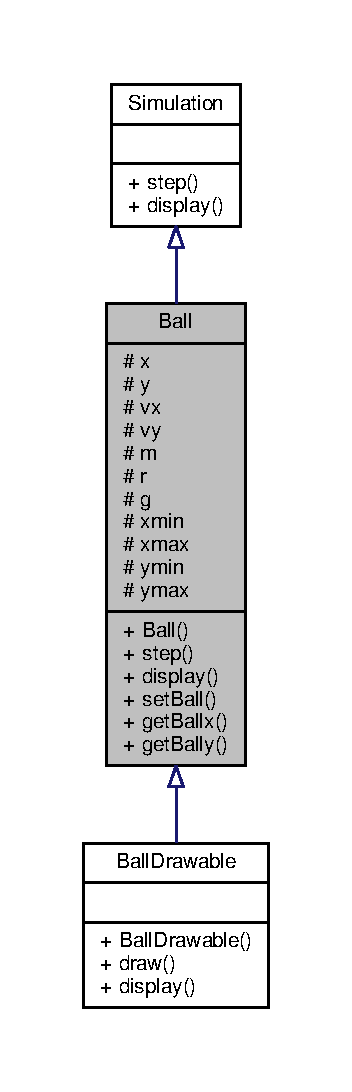
\includegraphics[width=169pt]{classBall__inherit__graph}
\end{center}
\end{figure}


Collaboration diagram for Ball\+:
\nopagebreak
\begin{figure}[H]
\begin{center}
\leavevmode
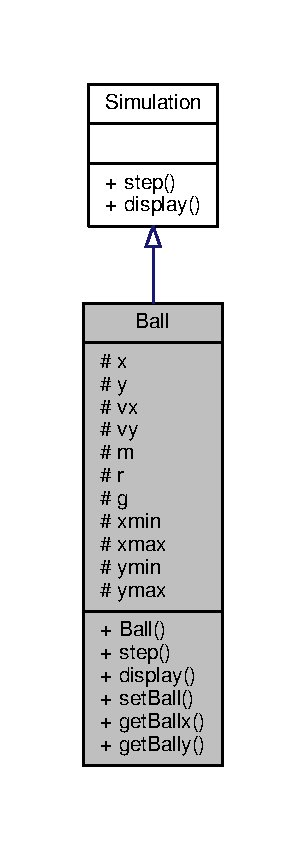
\includegraphics[width=147pt]{classBall__coll__graph}
\end{center}
\end{figure}
\subsection*{Public Member Functions}
\begin{DoxyCompactItemize}
\item 
\hyperlink{classBall_a86a144d3dad6c953e422e32435923bbb}{Ball} ()
\item 
void \hyperlink{classBall_a92dc65e1ed710ff01a4cbbb591ad7cb3}{step} (double dt)
\item 
void \hyperlink{classBall_a4a575db97fe36b3caa001ade4affeb18}{display} ()
\item 
double \hyperlink{classBall_a5de2a9c31906ebd899e51c6ddca7ef3a}{set\+Ball} (double xp, double yp)
\item 
double \hyperlink{classBall_a683551ec9c891d1420a1aab806bfef43}{get\+Ballx} ()
\item 
double \hyperlink{classBall_ae0b2224e6fbc8897ce132b229ceab446}{get\+Bally} ()
\end{DoxyCompactItemize}
\subsection*{Protected Attributes}
\begin{DoxyCompactItemize}
\item 
double \hyperlink{classBall_a60894aab5e27e93bacf2393b9110a049}{x}
\item 
double \hyperlink{classBall_a17d73231eab81d0e74cf28d0068fe5cb}{y}
\item 
double \hyperlink{classBall_a4cc3e6d17874d6a99d72657af3bd3a33}{vx}
\item 
double \hyperlink{classBall_aa58f7f56586df265f2fd1d56ce1f0504}{vy}
\item 
double \hyperlink{classBall_a78ecb2a76fb573ad0411b040dfc84e9d}{m}
\item 
double \hyperlink{classBall_aaf3fbb4a93f5efaa933ddd63976f73b5}{r}
\item 
double \hyperlink{classBall_a3573a38b1d3bac62a0bdf7060632bf98}{g}
\item 
double \hyperlink{classBall_ad100dde6b63de229a2bc86b9094526e1}{xmin}
\item 
double \hyperlink{classBall_ab31305d68cd9cd571f119dc9f78d394c}{xmax}
\item 
double \hyperlink{classBall_a01797d790fe45fc9294edece2ff72c5b}{ymin}
\item 
double \hyperlink{classBall_ada883fa45e2bc0cbcd04fec775bfcc89}{ymax}
\end{DoxyCompactItemize}


\subsection{Detailed Description}
file\+: \hyperlink{ball_8h}{ball.\+h} brief\+: \hyperlink{classBall}{Ball} class author\+: Andrea Vedaldi 

\subsection{Constructor \& Destructor Documentation}
\mbox{\Hypertarget{classBall_a86a144d3dad6c953e422e32435923bbb}\label{classBall_a86a144d3dad6c953e422e32435923bbb}} 
\index{Ball@{Ball}!Ball@{Ball}}
\index{Ball@{Ball}!Ball@{Ball}}
\subsubsection{\texorpdfstring{Ball()}{Ball()}}
{\footnotesize\ttfamily Ball\+::\+Ball (\begin{DoxyParamCaption}{ }\end{DoxyParamCaption})}

file\+: \hyperlink{ball_8cpp}{ball.\+cpp} brief\+: \hyperlink{classBall}{Ball} class -\/ implementation author\+: Andrea Vedaldi 

\subsection{Member Function Documentation}
\mbox{\Hypertarget{classBall_a4a575db97fe36b3caa001ade4affeb18}\label{classBall_a4a575db97fe36b3caa001ade4affeb18}} 
\index{Ball@{Ball}!display@{display}}
\index{display@{display}!Ball@{Ball}}
\subsubsection{\texorpdfstring{display()}{display()}}
{\footnotesize\ttfamily void Ball\+::display (\begin{DoxyParamCaption}{ }\end{DoxyParamCaption})\hspace{0.3cm}{\ttfamily [virtual]}}



Implements \hyperlink{classSimulation_a6f8e5272dbb5dea34970f0695419ff03}{Simulation}.



Reimplemented in \hyperlink{classBallDrawable_a934809e648474de989666d41a34a880e}{Ball\+Drawable}.

\mbox{\Hypertarget{classBall_a683551ec9c891d1420a1aab806bfef43}\label{classBall_a683551ec9c891d1420a1aab806bfef43}} 
\index{Ball@{Ball}!get\+Ballx@{get\+Ballx}}
\index{get\+Ballx@{get\+Ballx}!Ball@{Ball}}
\subsubsection{\texorpdfstring{get\+Ballx()}{getBallx()}}
{\footnotesize\ttfamily double Ball\+::get\+Ballx (\begin{DoxyParamCaption}{ }\end{DoxyParamCaption})}

\mbox{\Hypertarget{classBall_ae0b2224e6fbc8897ce132b229ceab446}\label{classBall_ae0b2224e6fbc8897ce132b229ceab446}} 
\index{Ball@{Ball}!get\+Bally@{get\+Bally}}
\index{get\+Bally@{get\+Bally}!Ball@{Ball}}
\subsubsection{\texorpdfstring{get\+Bally()}{getBally()}}
{\footnotesize\ttfamily double Ball\+::get\+Bally (\begin{DoxyParamCaption}{ }\end{DoxyParamCaption})}

\mbox{\Hypertarget{classBall_a5de2a9c31906ebd899e51c6ddca7ef3a}\label{classBall_a5de2a9c31906ebd899e51c6ddca7ef3a}} 
\index{Ball@{Ball}!set\+Ball@{set\+Ball}}
\index{set\+Ball@{set\+Ball}!Ball@{Ball}}
\subsubsection{\texorpdfstring{set\+Ball()}{setBall()}}
{\footnotesize\ttfamily double Ball\+::set\+Ball (\begin{DoxyParamCaption}\item[{double}]{xp,  }\item[{double}]{yp }\end{DoxyParamCaption})}

\mbox{\Hypertarget{classBall_a92dc65e1ed710ff01a4cbbb591ad7cb3}\label{classBall_a92dc65e1ed710ff01a4cbbb591ad7cb3}} 
\index{Ball@{Ball}!step@{step}}
\index{step@{step}!Ball@{Ball}}
\subsubsection{\texorpdfstring{step()}{step()}}
{\footnotesize\ttfamily void Ball\+::step (\begin{DoxyParamCaption}\item[{double}]{dt }\end{DoxyParamCaption})\hspace{0.3cm}{\ttfamily [virtual]}}



Implements \hyperlink{classSimulation_a1040e261c063e307871fb1dfe664fb0a}{Simulation}.



\subsection{Member Data Documentation}
\mbox{\Hypertarget{classBall_a3573a38b1d3bac62a0bdf7060632bf98}\label{classBall_a3573a38b1d3bac62a0bdf7060632bf98}} 
\index{Ball@{Ball}!g@{g}}
\index{g@{g}!Ball@{Ball}}
\subsubsection{\texorpdfstring{g}{g}}
{\footnotesize\ttfamily double Ball\+::g\hspace{0.3cm}{\ttfamily [protected]}}

\mbox{\Hypertarget{classBall_a78ecb2a76fb573ad0411b040dfc84e9d}\label{classBall_a78ecb2a76fb573ad0411b040dfc84e9d}} 
\index{Ball@{Ball}!m@{m}}
\index{m@{m}!Ball@{Ball}}
\subsubsection{\texorpdfstring{m}{m}}
{\footnotesize\ttfamily double Ball\+::m\hspace{0.3cm}{\ttfamily [protected]}}

\mbox{\Hypertarget{classBall_aaf3fbb4a93f5efaa933ddd63976f73b5}\label{classBall_aaf3fbb4a93f5efaa933ddd63976f73b5}} 
\index{Ball@{Ball}!r@{r}}
\index{r@{r}!Ball@{Ball}}
\subsubsection{\texorpdfstring{r}{r}}
{\footnotesize\ttfamily double Ball\+::r\hspace{0.3cm}{\ttfamily [protected]}}

\mbox{\Hypertarget{classBall_a4cc3e6d17874d6a99d72657af3bd3a33}\label{classBall_a4cc3e6d17874d6a99d72657af3bd3a33}} 
\index{Ball@{Ball}!vx@{vx}}
\index{vx@{vx}!Ball@{Ball}}
\subsubsection{\texorpdfstring{vx}{vx}}
{\footnotesize\ttfamily double Ball\+::vx\hspace{0.3cm}{\ttfamily [protected]}}

\mbox{\Hypertarget{classBall_aa58f7f56586df265f2fd1d56ce1f0504}\label{classBall_aa58f7f56586df265f2fd1d56ce1f0504}} 
\index{Ball@{Ball}!vy@{vy}}
\index{vy@{vy}!Ball@{Ball}}
\subsubsection{\texorpdfstring{vy}{vy}}
{\footnotesize\ttfamily double Ball\+::vy\hspace{0.3cm}{\ttfamily [protected]}}

\mbox{\Hypertarget{classBall_a60894aab5e27e93bacf2393b9110a049}\label{classBall_a60894aab5e27e93bacf2393b9110a049}} 
\index{Ball@{Ball}!x@{x}}
\index{x@{x}!Ball@{Ball}}
\subsubsection{\texorpdfstring{x}{x}}
{\footnotesize\ttfamily double Ball\+::x\hspace{0.3cm}{\ttfamily [protected]}}

\mbox{\Hypertarget{classBall_ab31305d68cd9cd571f119dc9f78d394c}\label{classBall_ab31305d68cd9cd571f119dc9f78d394c}} 
\index{Ball@{Ball}!xmax@{xmax}}
\index{xmax@{xmax}!Ball@{Ball}}
\subsubsection{\texorpdfstring{xmax}{xmax}}
{\footnotesize\ttfamily double Ball\+::xmax\hspace{0.3cm}{\ttfamily [protected]}}

\mbox{\Hypertarget{classBall_ad100dde6b63de229a2bc86b9094526e1}\label{classBall_ad100dde6b63de229a2bc86b9094526e1}} 
\index{Ball@{Ball}!xmin@{xmin}}
\index{xmin@{xmin}!Ball@{Ball}}
\subsubsection{\texorpdfstring{xmin}{xmin}}
{\footnotesize\ttfamily double Ball\+::xmin\hspace{0.3cm}{\ttfamily [protected]}}

\mbox{\Hypertarget{classBall_a17d73231eab81d0e74cf28d0068fe5cb}\label{classBall_a17d73231eab81d0e74cf28d0068fe5cb}} 
\index{Ball@{Ball}!y@{y}}
\index{y@{y}!Ball@{Ball}}
\subsubsection{\texorpdfstring{y}{y}}
{\footnotesize\ttfamily double Ball\+::y\hspace{0.3cm}{\ttfamily [protected]}}

\mbox{\Hypertarget{classBall_ada883fa45e2bc0cbcd04fec775bfcc89}\label{classBall_ada883fa45e2bc0cbcd04fec775bfcc89}} 
\index{Ball@{Ball}!ymax@{ymax}}
\index{ymax@{ymax}!Ball@{Ball}}
\subsubsection{\texorpdfstring{ymax}{ymax}}
{\footnotesize\ttfamily double Ball\+::ymax\hspace{0.3cm}{\ttfamily [protected]}}

\mbox{\Hypertarget{classBall_a01797d790fe45fc9294edece2ff72c5b}\label{classBall_a01797d790fe45fc9294edece2ff72c5b}} 
\index{Ball@{Ball}!ymin@{ymin}}
\index{ymin@{ymin}!Ball@{Ball}}
\subsubsection{\texorpdfstring{ymin}{ymin}}
{\footnotesize\ttfamily double Ball\+::ymin\hspace{0.3cm}{\ttfamily [protected]}}



The documentation for this class was generated from the following files\+:\begin{DoxyCompactItemize}
\item 
\hyperlink{ball_8h}{ball.\+h}\item 
\hyperlink{ball_8cpp}{ball.\+cpp}\end{DoxyCompactItemize}

\hypertarget{classBallDrawable}{}\section{Ball\+Drawable Class Reference}
\label{classBallDrawable}\index{Ball\+Drawable@{Ball\+Drawable}}


Inheritance diagram for Ball\+Drawable\+:
\nopagebreak
\begin{figure}[H]
\begin{center}
\leavevmode
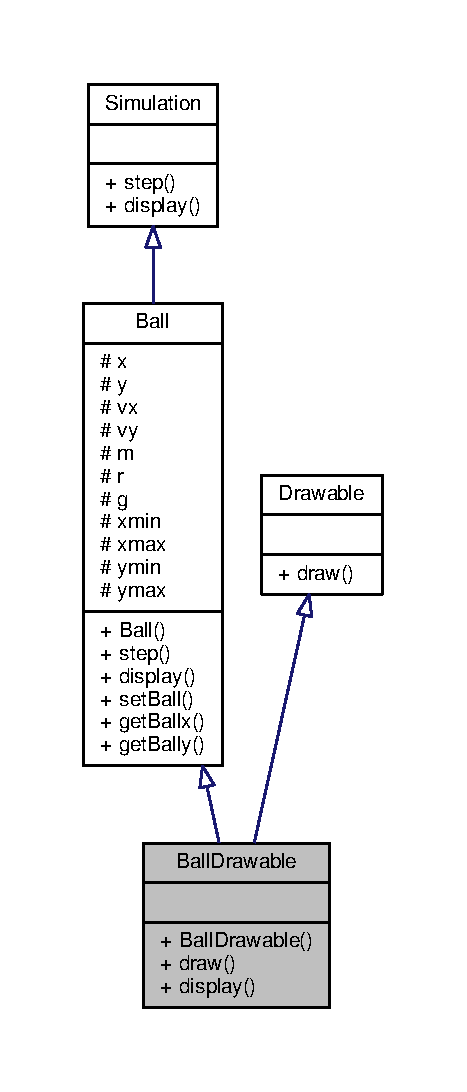
\includegraphics[width=224pt]{classBallDrawable__inherit__graph}
\end{center}
\end{figure}


Collaboration diagram for Ball\+Drawable\+:
\nopagebreak
\begin{figure}[H]
\begin{center}
\leavevmode
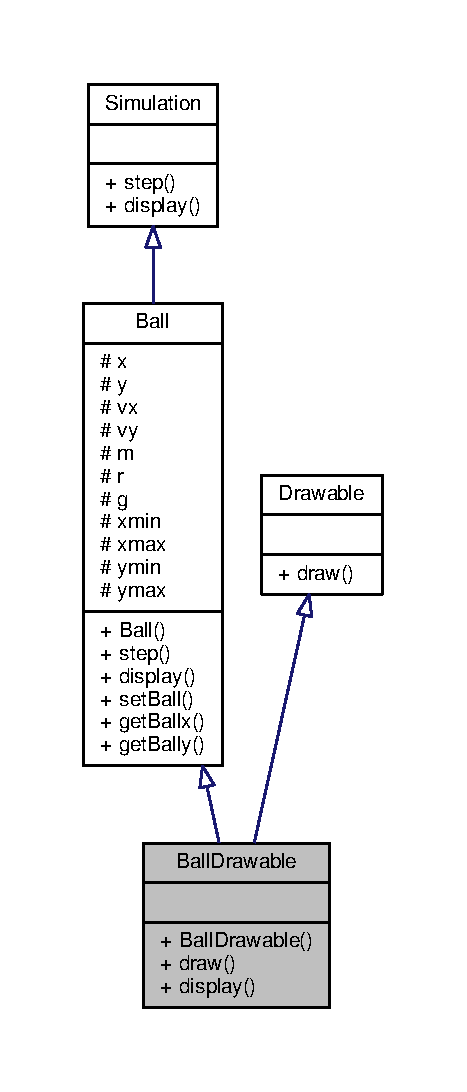
\includegraphics[width=224pt]{classBallDrawable__coll__graph}
\end{center}
\end{figure}
\subsection*{Public Member Functions}
\begin{DoxyCompactItemize}
\item 
\hyperlink{classBallDrawable_a50bda55f52c2ddbdf2bba8dde1471957}{Ball\+Drawable} ()
\item 
void \hyperlink{classBallDrawable_ae7cf6aaf513598338f14fc5c04bb7aed}{draw} ()
\item 
void \hyperlink{classBallDrawable_a934809e648474de989666d41a34a880e}{display} ()
\end{DoxyCompactItemize}
\subsection*{Additional Inherited Members}


\subsection{Detailed Description}
file\+: \hyperlink{test-ball-graphics_8cpp}{test-\/ball-\/graphics.\+cpp} brief\+: Tests the bouncing ball simulation with graphical output author\+: Andrea Vedaldi 

\subsection{Constructor \& Destructor Documentation}
\mbox{\Hypertarget{classBallDrawable_a50bda55f52c2ddbdf2bba8dde1471957}\label{classBallDrawable_a50bda55f52c2ddbdf2bba8dde1471957}} 
\index{Ball\+Drawable@{Ball\+Drawable}!Ball\+Drawable@{Ball\+Drawable}}
\index{Ball\+Drawable@{Ball\+Drawable}!Ball\+Drawable@{Ball\+Drawable}}
\subsubsection{\texorpdfstring{Ball\+Drawable()}{BallDrawable()}}
{\footnotesize\ttfamily Ball\+Drawable\+::\+Ball\+Drawable (\begin{DoxyParamCaption}{ }\end{DoxyParamCaption})\hspace{0.3cm}{\ttfamily [inline]}}



\subsection{Member Function Documentation}
\mbox{\Hypertarget{classBallDrawable_a934809e648474de989666d41a34a880e}\label{classBallDrawable_a934809e648474de989666d41a34a880e}} 
\index{Ball\+Drawable@{Ball\+Drawable}!display@{display}}
\index{display@{display}!Ball\+Drawable@{Ball\+Drawable}}
\subsubsection{\texorpdfstring{display()}{display()}}
{\footnotesize\ttfamily void Ball\+Drawable\+::display (\begin{DoxyParamCaption}{ }\end{DoxyParamCaption})\hspace{0.3cm}{\ttfamily [inline]}, {\ttfamily [virtual]}}



Reimplemented from \hyperlink{classBall_a4a575db97fe36b3caa001ade4affeb18}{Ball}.

\mbox{\Hypertarget{classBallDrawable_ae7cf6aaf513598338f14fc5c04bb7aed}\label{classBallDrawable_ae7cf6aaf513598338f14fc5c04bb7aed}} 
\index{Ball\+Drawable@{Ball\+Drawable}!draw@{draw}}
\index{draw@{draw}!Ball\+Drawable@{Ball\+Drawable}}
\subsubsection{\texorpdfstring{draw()}{draw()}}
{\footnotesize\ttfamily void Ball\+Drawable\+::draw (\begin{DoxyParamCaption}{ }\end{DoxyParamCaption})\hspace{0.3cm}{\ttfamily [inline]}, {\ttfamily [virtual]}}



Reimplemented from \hyperlink{classDrawable_a1231e00fe6022c2ff0e8d61fd23c5c23}{Drawable}.



The documentation for this class was generated from the following file\+:\begin{DoxyCompactItemize}
\item 
\hyperlink{test-ball-graphics_8cpp}{test-\/ball-\/graphics.\+cpp}\end{DoxyCompactItemize}

\hypertarget{classDrawable}{}\section{Drawable Class Reference}
\label{classDrawable}\index{Drawable@{Drawable}}


{\ttfamily \#include $<$graphics.\+h$>$}



Inheritance diagram for Drawable\+:
\nopagebreak
\begin{figure}[H]
\begin{center}
\leavevmode
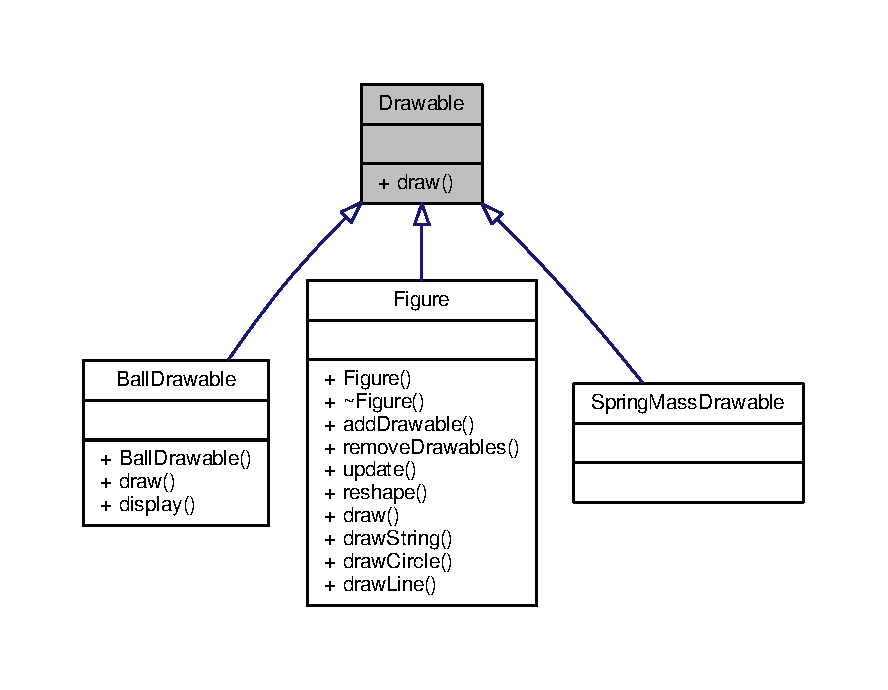
\includegraphics[width=350pt]{classDrawable__inherit__graph}
\end{center}
\end{figure}


Collaboration diagram for Drawable\+:
\nopagebreak
\begin{figure}[H]
\begin{center}
\leavevmode
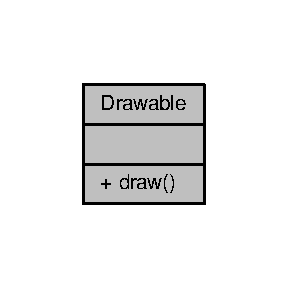
\includegraphics[width=138pt]{classDrawable__coll__graph}
\end{center}
\end{figure}
\subsection*{Public Member Functions}
\begin{DoxyCompactItemize}
\item 
virtual void \hyperlink{classDrawable_a1231e00fe6022c2ff0e8d61fd23c5c23}{draw} ()
\end{DoxyCompactItemize}


\subsection{Member Function Documentation}
\mbox{\Hypertarget{classDrawable_a1231e00fe6022c2ff0e8d61fd23c5c23}\label{classDrawable_a1231e00fe6022c2ff0e8d61fd23c5c23}} 
\index{Drawable@{Drawable}!draw@{draw}}
\index{draw@{draw}!Drawable@{Drawable}}
\subsubsection{\texorpdfstring{draw()}{draw()}}
{\footnotesize\ttfamily void Drawable\+::draw (\begin{DoxyParamCaption}{ }\end{DoxyParamCaption})\hspace{0.3cm}{\ttfamily [virtual]}}



Reimplemented in \hyperlink{classFigure_afb62fad838fc6f7ece4f88b318b5862a}{Figure}, and \hyperlink{classBallDrawable_ae7cf6aaf513598338f14fc5c04bb7aed}{Ball\+Drawable}.



The documentation for this class was generated from the following files\+:\begin{DoxyCompactItemize}
\item 
\hyperlink{graphics_8h}{graphics.\+h}\item 
\hyperlink{graphics_8cpp}{graphics.\+cpp}\end{DoxyCompactItemize}

\hypertarget{classFigure}{}\section{Figure Class Reference}
\label{classFigure}\index{Figure@{Figure}}


{\ttfamily \#include $<$graphics.\+h$>$}



Inheritance diagram for Figure\+:
\nopagebreak
\begin{figure}[H]
\begin{center}
\leavevmode
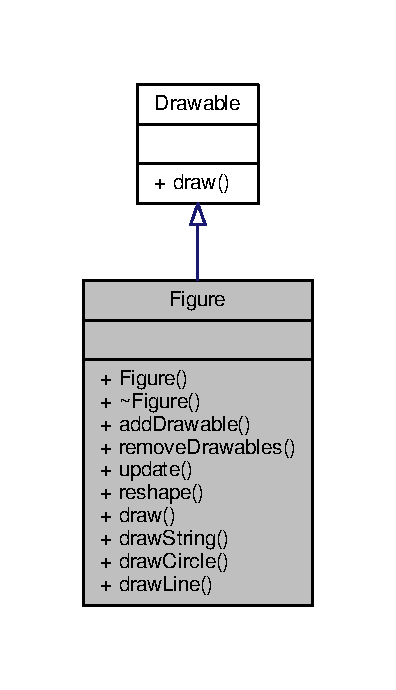
\includegraphics[width=190pt]{classFigure__inherit__graph}
\end{center}
\end{figure}


Collaboration diagram for Figure\+:
\nopagebreak
\begin{figure}[H]
\begin{center}
\leavevmode
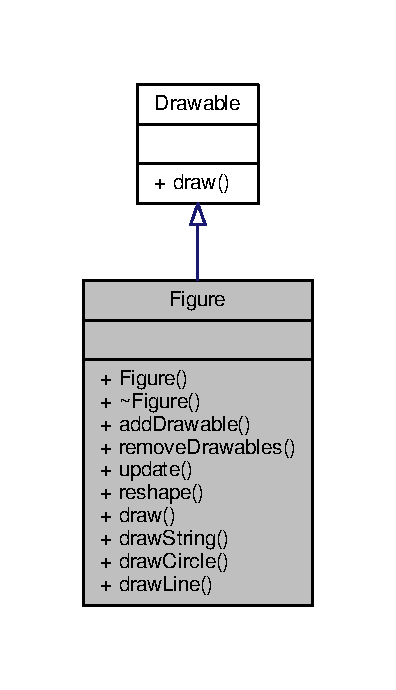
\includegraphics[width=190pt]{classFigure__coll__graph}
\end{center}
\end{figure}
\subsection*{Public Member Functions}
\begin{DoxyCompactItemize}
\item 
\hyperlink{classFigure_a9c58a51110b7035bb899035b15f6aa6d}{Figure} (std\+::string name)
\item 
\hyperlink{classFigure_af155c20558330034441de6a19d94f4a7}{$\sim$\+Figure} ()
\item 
void \hyperlink{classFigure_ac4960ce394966b1171c8ea49fb694cef}{add\+Drawable} (\hyperlink{classDrawable}{Drawable} $\ast$object)
\item 
void \hyperlink{classFigure_a6f239679543a9154ca1b6523094f7eae}{remove\+Drawables} (\hyperlink{classDrawable}{Drawable} $\ast$object)
\item 
void \hyperlink{classFigure_ac78a5c4997e27f48b40a2d86a4b92b9c}{update} () const
\item 
void \hyperlink{classFigure_a876db9bf0c44bcdcdac91f7d040d5f71}{reshape} (int width, int height)
\item 
void \hyperlink{classFigure_afb62fad838fc6f7ece4f88b318b5862a}{draw} ()
\item 
void \hyperlink{classFigure_a8d06d9d1a75b58c6f40881c0737bc5e2}{draw\+String} (double x, double y, std\+::string str)
\item 
void \hyperlink{classFigure_a7c99f033d2de6e1148bfd972610ad61b}{draw\+Circle} (double x, double y, double radius)
\item 
void \hyperlink{classFigure_ad5edf6262504de7c3c7eff6eb8be3c3e}{draw\+Line} (double x1, double y1, double x2, double y2, double thickness)
\end{DoxyCompactItemize}


\subsection{Constructor \& Destructor Documentation}
\mbox{\Hypertarget{classFigure_a9c58a51110b7035bb899035b15f6aa6d}\label{classFigure_a9c58a51110b7035bb899035b15f6aa6d}} 
\index{Figure@{Figure}!Figure@{Figure}}
\index{Figure@{Figure}!Figure@{Figure}}
\subsubsection{\texorpdfstring{Figure()}{Figure()}}
{\footnotesize\ttfamily Figure\+::\+Figure (\begin{DoxyParamCaption}\item[{std\+::string}]{name }\end{DoxyParamCaption})}

\mbox{\Hypertarget{classFigure_af155c20558330034441de6a19d94f4a7}\label{classFigure_af155c20558330034441de6a19d94f4a7}} 
\index{Figure@{Figure}!````~Figure@{$\sim$\+Figure}}
\index{````~Figure@{$\sim$\+Figure}!Figure@{Figure}}
\subsubsection{\texorpdfstring{$\sim$\+Figure()}{~Figure()}}
{\footnotesize\ttfamily Figure\+::$\sim$\+Figure (\begin{DoxyParamCaption}{ }\end{DoxyParamCaption})}



\subsection{Member Function Documentation}
\mbox{\Hypertarget{classFigure_ac4960ce394966b1171c8ea49fb694cef}\label{classFigure_ac4960ce394966b1171c8ea49fb694cef}} 
\index{Figure@{Figure}!add\+Drawable@{add\+Drawable}}
\index{add\+Drawable@{add\+Drawable}!Figure@{Figure}}
\subsubsection{\texorpdfstring{add\+Drawable()}{addDrawable()}}
{\footnotesize\ttfamily void Figure\+::add\+Drawable (\begin{DoxyParamCaption}\item[{\hyperlink{classDrawable}{Drawable} $\ast$}]{object }\end{DoxyParamCaption})}

\mbox{\Hypertarget{classFigure_afb62fad838fc6f7ece4f88b318b5862a}\label{classFigure_afb62fad838fc6f7ece4f88b318b5862a}} 
\index{Figure@{Figure}!draw@{draw}}
\index{draw@{draw}!Figure@{Figure}}
\subsubsection{\texorpdfstring{draw()}{draw()}}
{\footnotesize\ttfamily void Figure\+::draw (\begin{DoxyParamCaption}{ }\end{DoxyParamCaption})\hspace{0.3cm}{\ttfamily [virtual]}}



Reimplemented from \hyperlink{classDrawable_a1231e00fe6022c2ff0e8d61fd23c5c23}{Drawable}.

\mbox{\Hypertarget{classFigure_a7c99f033d2de6e1148bfd972610ad61b}\label{classFigure_a7c99f033d2de6e1148bfd972610ad61b}} 
\index{Figure@{Figure}!draw\+Circle@{draw\+Circle}}
\index{draw\+Circle@{draw\+Circle}!Figure@{Figure}}
\subsubsection{\texorpdfstring{draw\+Circle()}{drawCircle()}}
{\footnotesize\ttfamily void Figure\+::draw\+Circle (\begin{DoxyParamCaption}\item[{double}]{x,  }\item[{double}]{y,  }\item[{double}]{radius }\end{DoxyParamCaption})}

\mbox{\Hypertarget{classFigure_ad5edf6262504de7c3c7eff6eb8be3c3e}\label{classFigure_ad5edf6262504de7c3c7eff6eb8be3c3e}} 
\index{Figure@{Figure}!draw\+Line@{draw\+Line}}
\index{draw\+Line@{draw\+Line}!Figure@{Figure}}
\subsubsection{\texorpdfstring{draw\+Line()}{drawLine()}}
{\footnotesize\ttfamily void Figure\+::draw\+Line (\begin{DoxyParamCaption}\item[{double}]{x1,  }\item[{double}]{y1,  }\item[{double}]{x2,  }\item[{double}]{y2,  }\item[{double}]{thickness }\end{DoxyParamCaption})}

\mbox{\Hypertarget{classFigure_a8d06d9d1a75b58c6f40881c0737bc5e2}\label{classFigure_a8d06d9d1a75b58c6f40881c0737bc5e2}} 
\index{Figure@{Figure}!draw\+String@{draw\+String}}
\index{draw\+String@{draw\+String}!Figure@{Figure}}
\subsubsection{\texorpdfstring{draw\+String()}{drawString()}}
{\footnotesize\ttfamily void Figure\+::draw\+String (\begin{DoxyParamCaption}\item[{double}]{x,  }\item[{double}]{y,  }\item[{std\+::string}]{str }\end{DoxyParamCaption})}

\mbox{\Hypertarget{classFigure_a6f239679543a9154ca1b6523094f7eae}\label{classFigure_a6f239679543a9154ca1b6523094f7eae}} 
\index{Figure@{Figure}!remove\+Drawables@{remove\+Drawables}}
\index{remove\+Drawables@{remove\+Drawables}!Figure@{Figure}}
\subsubsection{\texorpdfstring{remove\+Drawables()}{removeDrawables()}}
{\footnotesize\ttfamily void Figure\+::remove\+Drawables (\begin{DoxyParamCaption}\item[{\hyperlink{classDrawable}{Drawable} $\ast$}]{object }\end{DoxyParamCaption})}

\mbox{\Hypertarget{classFigure_a876db9bf0c44bcdcdac91f7d040d5f71}\label{classFigure_a876db9bf0c44bcdcdac91f7d040d5f71}} 
\index{Figure@{Figure}!reshape@{reshape}}
\index{reshape@{reshape}!Figure@{Figure}}
\subsubsection{\texorpdfstring{reshape()}{reshape()}}
{\footnotesize\ttfamily void Figure\+::reshape (\begin{DoxyParamCaption}\item[{int}]{width,  }\item[{int}]{height }\end{DoxyParamCaption})}

\mbox{\Hypertarget{classFigure_ac78a5c4997e27f48b40a2d86a4b92b9c}\label{classFigure_ac78a5c4997e27f48b40a2d86a4b92b9c}} 
\index{Figure@{Figure}!update@{update}}
\index{update@{update}!Figure@{Figure}}
\subsubsection{\texorpdfstring{update()}{update()}}
{\footnotesize\ttfamily void Figure\+::update (\begin{DoxyParamCaption}{ }\end{DoxyParamCaption}) const}



The documentation for this class was generated from the following files\+:\begin{DoxyCompactItemize}
\item 
\hyperlink{graphics_8h}{graphics.\+h}\item 
\hyperlink{graphics_8cpp}{graphics.\+cpp}\end{DoxyCompactItemize}

\hypertarget{classMass}{}\section{Mass Class Reference}
\label{classMass}\index{Mass@{Mass}}


{\ttfamily \#include $<$springmass.\+h$>$}



Collaboration diagram for Mass\+:
\nopagebreak
\begin{figure}[H]
\begin{center}
\leavevmode
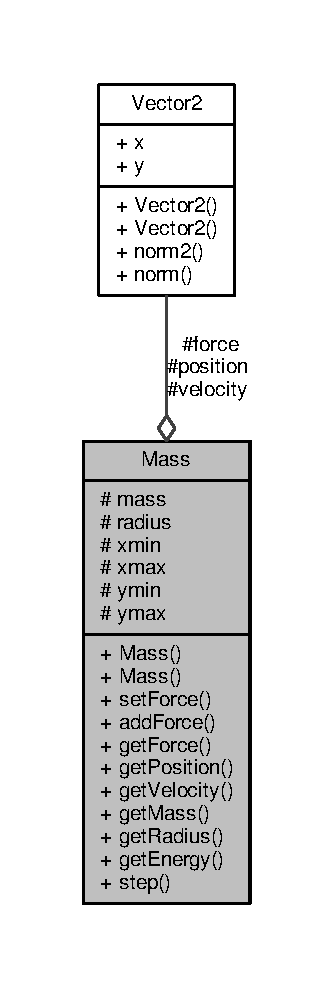
\includegraphics[width=160pt]{classMass__coll__graph}
\end{center}
\end{figure}
\subsection*{Public Member Functions}
\begin{DoxyCompactItemize}
\item 
\hyperlink{classMass_aa5d7017a4539bd4b76422cf193a0d23c}{Mass} ()
\item 
\hyperlink{classMass_adc27886a699de8add33229abb90a5469}{Mass} (\hyperlink{classVector2}{Vector2} \hyperlink{classMass_a6a0d58d24ab413d10d0cee1f3fb82bf7}{position}, \hyperlink{classVector2}{Vector2} \hyperlink{classMass_ab3825e4083083ba184e5060303b913a7}{velocity}, double \hyperlink{classMass_a8f37b93ded277000424b7a92adcf9c30}{mass}, double \hyperlink{classMass_afca87b38f7a4a6c4cfadbfba313dc4cf}{radius})
\item 
void \hyperlink{classMass_a0e1280cef830d9d160577fe3d46ac6f5}{set\+Force} (\hyperlink{classVector2}{Vector2} f)
\item 
void \hyperlink{classMass_aa4c034fd024e5ef2c81b4f9b5ff4ca7a}{add\+Force} (\hyperlink{classVector2}{Vector2} f)
\item 
\hyperlink{classVector2}{Vector2} \hyperlink{classMass_a41b3a36c1f242dd8a7018693de3a59bb}{get\+Force} () const
\item 
\hyperlink{classVector2}{Vector2} \hyperlink{classMass_a7b244f213544f309b07970e4883089dc}{get\+Position} () const
\item 
\hyperlink{classVector2}{Vector2} \hyperlink{classMass_adba409e1c341b4709a2545a354b8c91d}{get\+Velocity} () const
\item 
double \hyperlink{classMass_a99e1ec35c6095c90a4b631228f04900f}{get\+Mass} () const
\item 
double \hyperlink{classMass_a9ec88fcb850a603f9f9085cfe09796ee}{get\+Radius} () const
\item 
double \hyperlink{classMass_a5296c919bc09faea8152b8d40c66f92f}{get\+Energy} (double gravity) const
\item 
void \hyperlink{classMass_af603ce820dd8afd520a98d8ac4f00933}{step} (double dt)
\end{DoxyCompactItemize}
\subsection*{Protected Attributes}
\begin{DoxyCompactItemize}
\item 
\hyperlink{classVector2}{Vector2} \hyperlink{classMass_a6a0d58d24ab413d10d0cee1f3fb82bf7}{position}
\item 
\hyperlink{classVector2}{Vector2} \hyperlink{classMass_ab3825e4083083ba184e5060303b913a7}{velocity}
\item 
\hyperlink{classVector2}{Vector2} \hyperlink{classMass_a0e78a40a61856046fe535f49c66ba04c}{force}
\item 
double \hyperlink{classMass_a8f37b93ded277000424b7a92adcf9c30}{mass}
\item 
double \hyperlink{classMass_afca87b38f7a4a6c4cfadbfba313dc4cf}{radius}
\item 
double \hyperlink{classMass_ad8c92b972c0c32e382bdd180cef9fa37}{xmin}
\item 
double \hyperlink{classMass_a6f2faa75c028993b95f07db8acbe1816}{xmax}
\item 
double \hyperlink{classMass_a994eea18acef1ab497634ae6c45e627a}{ymin}
\item 
double \hyperlink{classMass_a2d5d2f1659dfc4b43096e6f5140114cc}{ymax}
\end{DoxyCompactItemize}


\subsection{Constructor \& Destructor Documentation}
\mbox{\Hypertarget{classMass_aa5d7017a4539bd4b76422cf193a0d23c}\label{classMass_aa5d7017a4539bd4b76422cf193a0d23c}} 
\index{Mass@{Mass}!Mass@{Mass}}
\index{Mass@{Mass}!Mass@{Mass}}
\subsubsection{\texorpdfstring{Mass()}{Mass()}\hspace{0.1cm}{\footnotesize\ttfamily [1/2]}}
{\footnotesize\ttfamily Mass\+::\+Mass (\begin{DoxyParamCaption}{ }\end{DoxyParamCaption})}

file\+: \hyperlink{springmass_8cpp}{springmass.\+cpp} brief\+: \hyperlink{classSpringMass}{Spring\+Mass} simulation implementation author\+: Andrea Vedaldi \mbox{\Hypertarget{classMass_adc27886a699de8add33229abb90a5469}\label{classMass_adc27886a699de8add33229abb90a5469}} 
\index{Mass@{Mass}!Mass@{Mass}}
\index{Mass@{Mass}!Mass@{Mass}}
\subsubsection{\texorpdfstring{Mass()}{Mass()}\hspace{0.1cm}{\footnotesize\ttfamily [2/2]}}
{\footnotesize\ttfamily Mass\+::\+Mass (\begin{DoxyParamCaption}\item[{\hyperlink{classVector2}{Vector2}}]{position,  }\item[{\hyperlink{classVector2}{Vector2}}]{velocity,  }\item[{double}]{mass,  }\item[{double}]{radius }\end{DoxyParamCaption})}



\subsection{Member Function Documentation}
\mbox{\Hypertarget{classMass_aa4c034fd024e5ef2c81b4f9b5ff4ca7a}\label{classMass_aa4c034fd024e5ef2c81b4f9b5ff4ca7a}} 
\index{Mass@{Mass}!add\+Force@{add\+Force}}
\index{add\+Force@{add\+Force}!Mass@{Mass}}
\subsubsection{\texorpdfstring{add\+Force()}{addForce()}}
{\footnotesize\ttfamily void Mass\+::add\+Force (\begin{DoxyParamCaption}\item[{\hyperlink{classVector2}{Vector2}}]{f }\end{DoxyParamCaption})}

\mbox{\Hypertarget{classMass_a5296c919bc09faea8152b8d40c66f92f}\label{classMass_a5296c919bc09faea8152b8d40c66f92f}} 
\index{Mass@{Mass}!get\+Energy@{get\+Energy}}
\index{get\+Energy@{get\+Energy}!Mass@{Mass}}
\subsubsection{\texorpdfstring{get\+Energy()}{getEnergy()}}
{\footnotesize\ttfamily double Mass\+::get\+Energy (\begin{DoxyParamCaption}\item[{double}]{gravity }\end{DoxyParamCaption}) const}

\mbox{\Hypertarget{classMass_a41b3a36c1f242dd8a7018693de3a59bb}\label{classMass_a41b3a36c1f242dd8a7018693de3a59bb}} 
\index{Mass@{Mass}!get\+Force@{get\+Force}}
\index{get\+Force@{get\+Force}!Mass@{Mass}}
\subsubsection{\texorpdfstring{get\+Force()}{getForce()}}
{\footnotesize\ttfamily \hyperlink{classVector2}{Vector2} Mass\+::get\+Force (\begin{DoxyParamCaption}{ }\end{DoxyParamCaption}) const}

\mbox{\Hypertarget{classMass_a99e1ec35c6095c90a4b631228f04900f}\label{classMass_a99e1ec35c6095c90a4b631228f04900f}} 
\index{Mass@{Mass}!get\+Mass@{get\+Mass}}
\index{get\+Mass@{get\+Mass}!Mass@{Mass}}
\subsubsection{\texorpdfstring{get\+Mass()}{getMass()}}
{\footnotesize\ttfamily double Mass\+::get\+Mass (\begin{DoxyParamCaption}{ }\end{DoxyParamCaption}) const}

\mbox{\Hypertarget{classMass_a7b244f213544f309b07970e4883089dc}\label{classMass_a7b244f213544f309b07970e4883089dc}} 
\index{Mass@{Mass}!get\+Position@{get\+Position}}
\index{get\+Position@{get\+Position}!Mass@{Mass}}
\subsubsection{\texorpdfstring{get\+Position()}{getPosition()}}
{\footnotesize\ttfamily \hyperlink{classVector2}{Vector2} Mass\+::get\+Position (\begin{DoxyParamCaption}{ }\end{DoxyParamCaption}) const}

\mbox{\Hypertarget{classMass_a9ec88fcb850a603f9f9085cfe09796ee}\label{classMass_a9ec88fcb850a603f9f9085cfe09796ee}} 
\index{Mass@{Mass}!get\+Radius@{get\+Radius}}
\index{get\+Radius@{get\+Radius}!Mass@{Mass}}
\subsubsection{\texorpdfstring{get\+Radius()}{getRadius()}}
{\footnotesize\ttfamily double Mass\+::get\+Radius (\begin{DoxyParamCaption}{ }\end{DoxyParamCaption}) const}

\mbox{\Hypertarget{classMass_adba409e1c341b4709a2545a354b8c91d}\label{classMass_adba409e1c341b4709a2545a354b8c91d}} 
\index{Mass@{Mass}!get\+Velocity@{get\+Velocity}}
\index{get\+Velocity@{get\+Velocity}!Mass@{Mass}}
\subsubsection{\texorpdfstring{get\+Velocity()}{getVelocity()}}
{\footnotesize\ttfamily \hyperlink{classVector2}{Vector2} Mass\+::get\+Velocity (\begin{DoxyParamCaption}{ }\end{DoxyParamCaption}) const}

\mbox{\Hypertarget{classMass_a0e1280cef830d9d160577fe3d46ac6f5}\label{classMass_a0e1280cef830d9d160577fe3d46ac6f5}} 
\index{Mass@{Mass}!set\+Force@{set\+Force}}
\index{set\+Force@{set\+Force}!Mass@{Mass}}
\subsubsection{\texorpdfstring{set\+Force()}{setForce()}}
{\footnotesize\ttfamily void Mass\+::set\+Force (\begin{DoxyParamCaption}\item[{\hyperlink{classVector2}{Vector2}}]{f }\end{DoxyParamCaption})}

\mbox{\Hypertarget{classMass_af603ce820dd8afd520a98d8ac4f00933}\label{classMass_af603ce820dd8afd520a98d8ac4f00933}} 
\index{Mass@{Mass}!step@{step}}
\index{step@{step}!Mass@{Mass}}
\subsubsection{\texorpdfstring{step()}{step()}}
{\footnotesize\ttfamily void Mass\+::step (\begin{DoxyParamCaption}\item[{double}]{dt }\end{DoxyParamCaption})}



\subsection{Member Data Documentation}
\mbox{\Hypertarget{classMass_a0e78a40a61856046fe535f49c66ba04c}\label{classMass_a0e78a40a61856046fe535f49c66ba04c}} 
\index{Mass@{Mass}!force@{force}}
\index{force@{force}!Mass@{Mass}}
\subsubsection{\texorpdfstring{force}{force}}
{\footnotesize\ttfamily \hyperlink{classVector2}{Vector2} Mass\+::force\hspace{0.3cm}{\ttfamily [protected]}}

\mbox{\Hypertarget{classMass_a8f37b93ded277000424b7a92adcf9c30}\label{classMass_a8f37b93ded277000424b7a92adcf9c30}} 
\index{Mass@{Mass}!mass@{mass}}
\index{mass@{mass}!Mass@{Mass}}
\subsubsection{\texorpdfstring{mass}{mass}}
{\footnotesize\ttfamily double Mass\+::mass\hspace{0.3cm}{\ttfamily [protected]}}

\mbox{\Hypertarget{classMass_a6a0d58d24ab413d10d0cee1f3fb82bf7}\label{classMass_a6a0d58d24ab413d10d0cee1f3fb82bf7}} 
\index{Mass@{Mass}!position@{position}}
\index{position@{position}!Mass@{Mass}}
\subsubsection{\texorpdfstring{position}{position}}
{\footnotesize\ttfamily \hyperlink{classVector2}{Vector2} Mass\+::position\hspace{0.3cm}{\ttfamily [protected]}}

\mbox{\Hypertarget{classMass_afca87b38f7a4a6c4cfadbfba313dc4cf}\label{classMass_afca87b38f7a4a6c4cfadbfba313dc4cf}} 
\index{Mass@{Mass}!radius@{radius}}
\index{radius@{radius}!Mass@{Mass}}
\subsubsection{\texorpdfstring{radius}{radius}}
{\footnotesize\ttfamily double Mass\+::radius\hspace{0.3cm}{\ttfamily [protected]}}

\mbox{\Hypertarget{classMass_ab3825e4083083ba184e5060303b913a7}\label{classMass_ab3825e4083083ba184e5060303b913a7}} 
\index{Mass@{Mass}!velocity@{velocity}}
\index{velocity@{velocity}!Mass@{Mass}}
\subsubsection{\texorpdfstring{velocity}{velocity}}
{\footnotesize\ttfamily \hyperlink{classVector2}{Vector2} Mass\+::velocity\hspace{0.3cm}{\ttfamily [protected]}}

\mbox{\Hypertarget{classMass_a6f2faa75c028993b95f07db8acbe1816}\label{classMass_a6f2faa75c028993b95f07db8acbe1816}} 
\index{Mass@{Mass}!xmax@{xmax}}
\index{xmax@{xmax}!Mass@{Mass}}
\subsubsection{\texorpdfstring{xmax}{xmax}}
{\footnotesize\ttfamily double Mass\+::xmax\hspace{0.3cm}{\ttfamily [protected]}}

\mbox{\Hypertarget{classMass_ad8c92b972c0c32e382bdd180cef9fa37}\label{classMass_ad8c92b972c0c32e382bdd180cef9fa37}} 
\index{Mass@{Mass}!xmin@{xmin}}
\index{xmin@{xmin}!Mass@{Mass}}
\subsubsection{\texorpdfstring{xmin}{xmin}}
{\footnotesize\ttfamily double Mass\+::xmin\hspace{0.3cm}{\ttfamily [protected]}}

\mbox{\Hypertarget{classMass_a2d5d2f1659dfc4b43096e6f5140114cc}\label{classMass_a2d5d2f1659dfc4b43096e6f5140114cc}} 
\index{Mass@{Mass}!ymax@{ymax}}
\index{ymax@{ymax}!Mass@{Mass}}
\subsubsection{\texorpdfstring{ymax}{ymax}}
{\footnotesize\ttfamily double Mass\+::ymax\hspace{0.3cm}{\ttfamily [protected]}}

\mbox{\Hypertarget{classMass_a994eea18acef1ab497634ae6c45e627a}\label{classMass_a994eea18acef1ab497634ae6c45e627a}} 
\index{Mass@{Mass}!ymin@{ymin}}
\index{ymin@{ymin}!Mass@{Mass}}
\subsubsection{\texorpdfstring{ymin}{ymin}}
{\footnotesize\ttfamily double Mass\+::ymin\hspace{0.3cm}{\ttfamily [protected]}}



The documentation for this class was generated from the following files\+:\begin{DoxyCompactItemize}
\item 
\hyperlink{springmass_8h}{springmass.\+h}\item 
\hyperlink{springmass_8cpp}{springmass.\+cpp}\end{DoxyCompactItemize}

\hypertarget{classSimulation}{}\section{Simulation Class Reference}
\label{classSimulation}\index{Simulation@{Simulation}}


{\ttfamily \#include $<$simulation.\+h$>$}



Inheritance diagram for Simulation\+:
\nopagebreak
\begin{figure}[H]
\begin{center}
\leavevmode
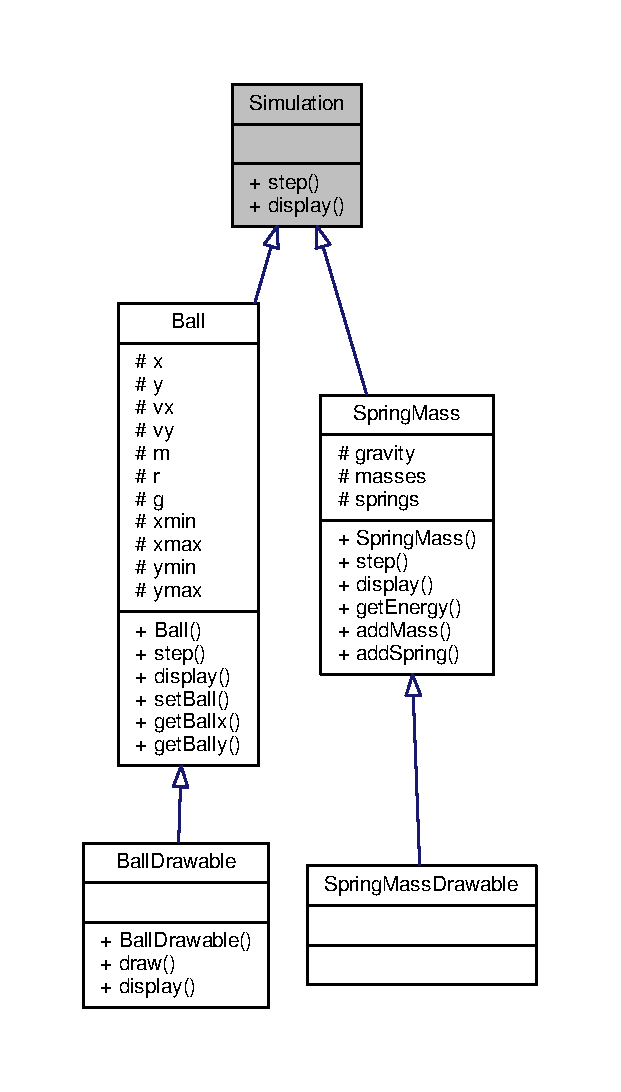
\includegraphics[width=298pt]{classSimulation__inherit__graph}
\end{center}
\end{figure}


Collaboration diagram for Simulation\+:
\nopagebreak
\begin{figure}[H]
\begin{center}
\leavevmode
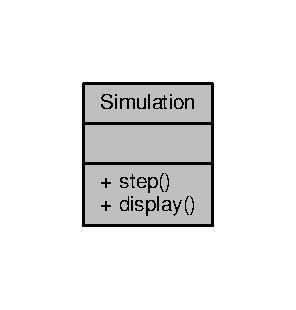
\includegraphics[width=142pt]{classSimulation__coll__graph}
\end{center}
\end{figure}
\subsection*{Public Member Functions}
\begin{DoxyCompactItemize}
\item 
virtual void \hyperlink{classSimulation_a1040e261c063e307871fb1dfe664fb0a}{step} (double dt)=0
\item 
virtual void \hyperlink{classSimulation_a6f8e5272dbb5dea34970f0695419ff03}{display} ()=0
\end{DoxyCompactItemize}


\subsection{Detailed Description}
file\+: \hyperlink{simulation_8h}{simulation.\+h} brief\+: \hyperlink{classSimulation}{Simulation} class (an interface) author\+: Andrea Vedaldi 

\subsection{Member Function Documentation}
\mbox{\Hypertarget{classSimulation_a6f8e5272dbb5dea34970f0695419ff03}\label{classSimulation_a6f8e5272dbb5dea34970f0695419ff03}} 
\index{Simulation@{Simulation}!display@{display}}
\index{display@{display}!Simulation@{Simulation}}
\subsubsection{\texorpdfstring{display()}{display()}}
{\footnotesize\ttfamily virtual void Simulation\+::display (\begin{DoxyParamCaption}{ }\end{DoxyParamCaption})\hspace{0.3cm}{\ttfamily [pure virtual]}}



Implemented in \hyperlink{classSpringMass_a97dc8e01e829e466198b3a8c201a5b13}{Spring\+Mass}, \hyperlink{classBallDrawable_a934809e648474de989666d41a34a880e}{Ball\+Drawable}, and \hyperlink{classBall_a4a575db97fe36b3caa001ade4affeb18}{Ball}.

\mbox{\Hypertarget{classSimulation_a1040e261c063e307871fb1dfe664fb0a}\label{classSimulation_a1040e261c063e307871fb1dfe664fb0a}} 
\index{Simulation@{Simulation}!step@{step}}
\index{step@{step}!Simulation@{Simulation}}
\subsubsection{\texorpdfstring{step()}{step()}}
{\footnotesize\ttfamily virtual void Simulation\+::step (\begin{DoxyParamCaption}\item[{double}]{dt }\end{DoxyParamCaption})\hspace{0.3cm}{\ttfamily [pure virtual]}}



Implemented in \hyperlink{classSpringMass_a187503b09da458570891a38612864e75}{Spring\+Mass}, and \hyperlink{classBall_a92dc65e1ed710ff01a4cbbb591ad7cb3}{Ball}.



The documentation for this class was generated from the following file\+:\begin{DoxyCompactItemize}
\item 
\hyperlink{simulation_8h}{simulation.\+h}\end{DoxyCompactItemize}

\hypertarget{classSpring}{}\section{Spring Class Reference}
\label{classSpring}\index{Spring@{Spring}}


{\ttfamily \#include $<$springmass.\+h$>$}



Collaboration diagram for Spring\+:
\nopagebreak
\begin{figure}[H]
\begin{center}
\leavevmode
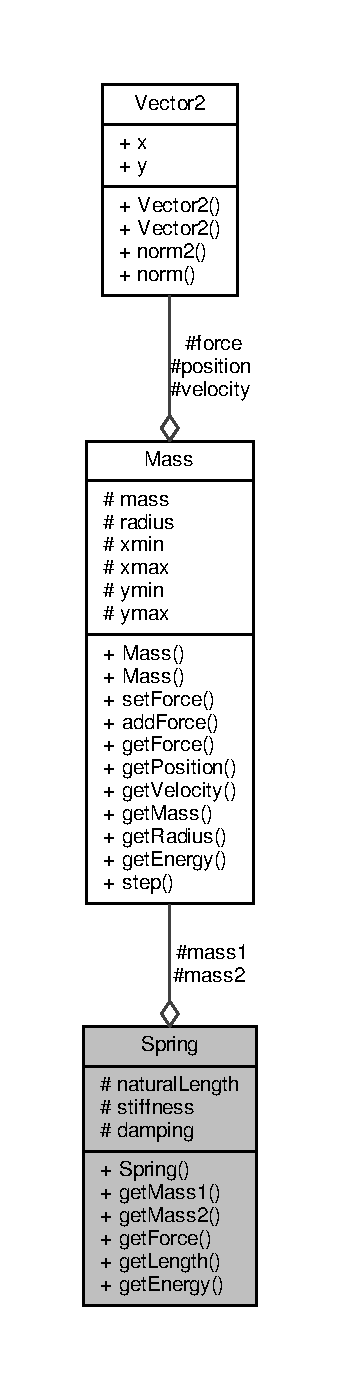
\includegraphics[height=550pt]{classSpring__coll__graph}
\end{center}
\end{figure}
\subsection*{Public Member Functions}
\begin{DoxyCompactItemize}
\item 
\hyperlink{classSpring_aa200d0ef9f53cf415c564e711079a5d9}{Spring} (\hyperlink{classMass}{Mass} $\ast$\hyperlink{classSpring_ab89136b001acfb27f95271781651c7f2}{mass1}, \hyperlink{classMass}{Mass} $\ast$\hyperlink{classSpring_af687f55d26b9799e7d7348104843855c}{mass2}, double \hyperlink{classSpring_a2b0a17c4655fda4b082289f5ff867197}{natural\+Length}, double \hyperlink{classSpring_aed22a149191c40dcef27af3e029e60fd}{stiffness}, double \hyperlink{classSpring_a3f82602a9f227c354d537fbf6c0344ec}{damping}=0.\+01)
\item 
\hyperlink{classMass}{Mass} $\ast$ \hyperlink{classSpring_af5b4786fc1829f556755c390a7c461bc}{get\+Mass1} () const
\item 
\hyperlink{classMass}{Mass} $\ast$ \hyperlink{classSpring_abcb4acf6d6f01eeff3b20c59674c05d3}{get\+Mass2} () const
\item 
\hyperlink{classVector2}{Vector2} \hyperlink{classSpring_a9b4eb2edf28f7d03f5acc7f8d276207f}{get\+Force} () const
\item 
double \hyperlink{classSpring_abac33a6e28978c4b09cee7f4709b9387}{get\+Length} () const
\item 
double \hyperlink{classSpring_a58ef4f35d8a552adb76662b4d7615741}{get\+Energy} () const
\end{DoxyCompactItemize}
\subsection*{Protected Attributes}
\begin{DoxyCompactItemize}
\item 
double \hyperlink{classSpring_a2b0a17c4655fda4b082289f5ff867197}{natural\+Length}
\item 
double \hyperlink{classSpring_aed22a149191c40dcef27af3e029e60fd}{stiffness}
\item 
double \hyperlink{classSpring_a3f82602a9f227c354d537fbf6c0344ec}{damping}
\item 
\hyperlink{classMass}{Mass} $\ast$ \hyperlink{classSpring_ab89136b001acfb27f95271781651c7f2}{mass1}
\item 
\hyperlink{classMass}{Mass} $\ast$ \hyperlink{classSpring_af687f55d26b9799e7d7348104843855c}{mass2}
\end{DoxyCompactItemize}


\subsection{Constructor \& Destructor Documentation}
\mbox{\Hypertarget{classSpring_aa200d0ef9f53cf415c564e711079a5d9}\label{classSpring_aa200d0ef9f53cf415c564e711079a5d9}} 
\index{Spring@{Spring}!Spring@{Spring}}
\index{Spring@{Spring}!Spring@{Spring}}
\subsubsection{\texorpdfstring{Spring()}{Spring()}}
{\footnotesize\ttfamily Spring\+::\+Spring (\begin{DoxyParamCaption}\item[{\hyperlink{classMass}{Mass} $\ast$}]{mass1,  }\item[{\hyperlink{classMass}{Mass} $\ast$}]{mass2,  }\item[{double}]{natural\+Length,  }\item[{double}]{stiffness,  }\item[{double}]{damping = {\ttfamily 0.01} }\end{DoxyParamCaption})}



\subsection{Member Function Documentation}
\mbox{\Hypertarget{classSpring_a58ef4f35d8a552adb76662b4d7615741}\label{classSpring_a58ef4f35d8a552adb76662b4d7615741}} 
\index{Spring@{Spring}!get\+Energy@{get\+Energy}}
\index{get\+Energy@{get\+Energy}!Spring@{Spring}}
\subsubsection{\texorpdfstring{get\+Energy()}{getEnergy()}}
{\footnotesize\ttfamily double Spring\+::get\+Energy (\begin{DoxyParamCaption}{ }\end{DoxyParamCaption}) const}

\mbox{\Hypertarget{classSpring_a9b4eb2edf28f7d03f5acc7f8d276207f}\label{classSpring_a9b4eb2edf28f7d03f5acc7f8d276207f}} 
\index{Spring@{Spring}!get\+Force@{get\+Force}}
\index{get\+Force@{get\+Force}!Spring@{Spring}}
\subsubsection{\texorpdfstring{get\+Force()}{getForce()}}
{\footnotesize\ttfamily \hyperlink{classVector2}{Vector2} Spring\+::get\+Force (\begin{DoxyParamCaption}{ }\end{DoxyParamCaption}) const}

\mbox{\Hypertarget{classSpring_abac33a6e28978c4b09cee7f4709b9387}\label{classSpring_abac33a6e28978c4b09cee7f4709b9387}} 
\index{Spring@{Spring}!get\+Length@{get\+Length}}
\index{get\+Length@{get\+Length}!Spring@{Spring}}
\subsubsection{\texorpdfstring{get\+Length()}{getLength()}}
{\footnotesize\ttfamily double Spring\+::get\+Length (\begin{DoxyParamCaption}{ }\end{DoxyParamCaption}) const}

\mbox{\Hypertarget{classSpring_af5b4786fc1829f556755c390a7c461bc}\label{classSpring_af5b4786fc1829f556755c390a7c461bc}} 
\index{Spring@{Spring}!get\+Mass1@{get\+Mass1}}
\index{get\+Mass1@{get\+Mass1}!Spring@{Spring}}
\subsubsection{\texorpdfstring{get\+Mass1()}{getMass1()}}
{\footnotesize\ttfamily \hyperlink{classMass}{Mass} $\ast$ Spring\+::get\+Mass1 (\begin{DoxyParamCaption}{ }\end{DoxyParamCaption}) const}

\mbox{\Hypertarget{classSpring_abcb4acf6d6f01eeff3b20c59674c05d3}\label{classSpring_abcb4acf6d6f01eeff3b20c59674c05d3}} 
\index{Spring@{Spring}!get\+Mass2@{get\+Mass2}}
\index{get\+Mass2@{get\+Mass2}!Spring@{Spring}}
\subsubsection{\texorpdfstring{get\+Mass2()}{getMass2()}}
{\footnotesize\ttfamily \hyperlink{classMass}{Mass} $\ast$ Spring\+::get\+Mass2 (\begin{DoxyParamCaption}{ }\end{DoxyParamCaption}) const}



\subsection{Member Data Documentation}
\mbox{\Hypertarget{classSpring_a3f82602a9f227c354d537fbf6c0344ec}\label{classSpring_a3f82602a9f227c354d537fbf6c0344ec}} 
\index{Spring@{Spring}!damping@{damping}}
\index{damping@{damping}!Spring@{Spring}}
\subsubsection{\texorpdfstring{damping}{damping}}
{\footnotesize\ttfamily double Spring\+::damping\hspace{0.3cm}{\ttfamily [protected]}}

\mbox{\Hypertarget{classSpring_ab89136b001acfb27f95271781651c7f2}\label{classSpring_ab89136b001acfb27f95271781651c7f2}} 
\index{Spring@{Spring}!mass1@{mass1}}
\index{mass1@{mass1}!Spring@{Spring}}
\subsubsection{\texorpdfstring{mass1}{mass1}}
{\footnotesize\ttfamily \hyperlink{classMass}{Mass}$\ast$ Spring\+::mass1\hspace{0.3cm}{\ttfamily [protected]}}

\mbox{\Hypertarget{classSpring_af687f55d26b9799e7d7348104843855c}\label{classSpring_af687f55d26b9799e7d7348104843855c}} 
\index{Spring@{Spring}!mass2@{mass2}}
\index{mass2@{mass2}!Spring@{Spring}}
\subsubsection{\texorpdfstring{mass2}{mass2}}
{\footnotesize\ttfamily \hyperlink{classMass}{Mass}$\ast$ Spring\+::mass2\hspace{0.3cm}{\ttfamily [protected]}}

\mbox{\Hypertarget{classSpring_a2b0a17c4655fda4b082289f5ff867197}\label{classSpring_a2b0a17c4655fda4b082289f5ff867197}} 
\index{Spring@{Spring}!natural\+Length@{natural\+Length}}
\index{natural\+Length@{natural\+Length}!Spring@{Spring}}
\subsubsection{\texorpdfstring{natural\+Length}{naturalLength}}
{\footnotesize\ttfamily double Spring\+::natural\+Length\hspace{0.3cm}{\ttfamily [protected]}}

\mbox{\Hypertarget{classSpring_aed22a149191c40dcef27af3e029e60fd}\label{classSpring_aed22a149191c40dcef27af3e029e60fd}} 
\index{Spring@{Spring}!stiffness@{stiffness}}
\index{stiffness@{stiffness}!Spring@{Spring}}
\subsubsection{\texorpdfstring{stiffness}{stiffness}}
{\footnotesize\ttfamily double Spring\+::stiffness\hspace{0.3cm}{\ttfamily [protected]}}



The documentation for this class was generated from the following files\+:\begin{DoxyCompactItemize}
\item 
\hyperlink{springmass_8h}{springmass.\+h}\item 
\hyperlink{springmass_8cpp}{springmass.\+cpp}\end{DoxyCompactItemize}

\hypertarget{classSpringMass}{}\section{Spring\+Mass Class Reference}
\label{classSpringMass}\index{Spring\+Mass@{Spring\+Mass}}


{\ttfamily \#include $<$springmass.\+h$>$}



Inheritance diagram for Spring\+Mass\+:
\nopagebreak
\begin{figure}[H]
\begin{center}
\leavevmode
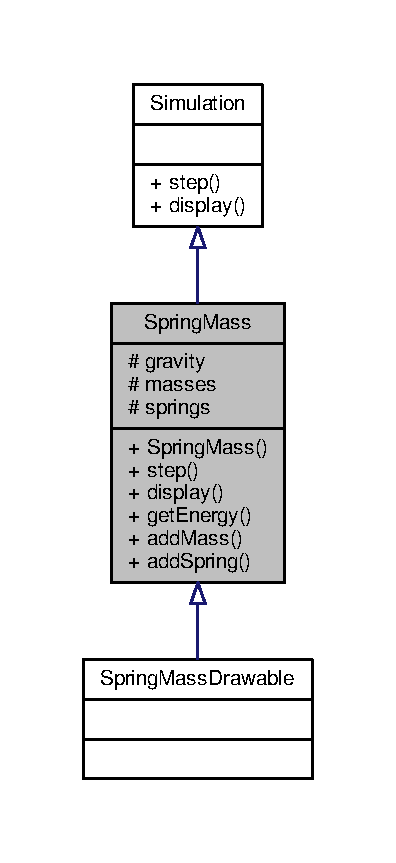
\includegraphics[width=190pt]{classSpringMass__inherit__graph}
\end{center}
\end{figure}


Collaboration diagram for Spring\+Mass\+:
\nopagebreak
\begin{figure}[H]
\begin{center}
\leavevmode
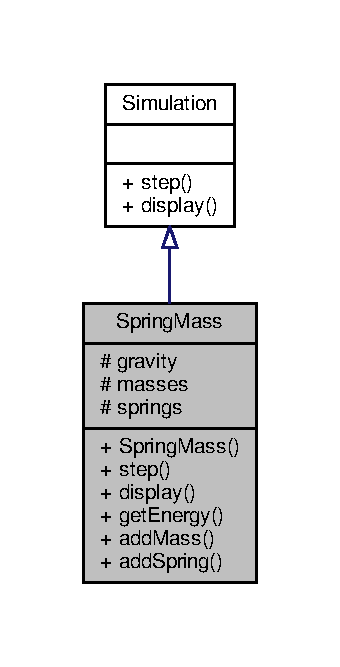
\includegraphics[width=163pt]{classSpringMass__coll__graph}
\end{center}
\end{figure}
\subsection*{Public Member Functions}
\begin{DoxyCompactItemize}
\item 
\hyperlink{classSpringMass_a5c94ec5d3adf73a7b3b7e9dd10045132}{Spring\+Mass} (double \hyperlink{classSpringMass_a8153c487713e1eea29caf109bc49e373}{gravity}=\hyperlink{springmass_8h_a03ad3bae72a0ac7965460a63fd454f44}{M\+O\+O\+N\+\_\+\+G\+R\+A\+V\+I\+TY})
\item 
void \hyperlink{classSpringMass_a187503b09da458570891a38612864e75}{step} (double dt)
\item 
void \hyperlink{classSpringMass_a97dc8e01e829e466198b3a8c201a5b13}{display} ()
\item 
double \hyperlink{classSpringMass_a1700091076aa83fff57fdec6876bf138}{get\+Energy} () const
\item 
int \hyperlink{classSpringMass_ac5185db5ea4078e3af82b7031d893302}{add\+Mass} (\hyperlink{classMass}{Mass} m)
\item 
void \hyperlink{classSpringMass_a61799a4987d64402de52f3772b68e8b2}{add\+Spring} (int i, int j, double length, double stiffness)
\end{DoxyCompactItemize}
\subsection*{Protected Types}
\begin{DoxyCompactItemize}
\item 
typedef std\+::vector$<$ \hyperlink{classMass}{Mass} $>$ \hyperlink{classSpringMass_a4871d5df726e2e6b656d1b1c5fdfecbe}{masses\+\_\+t}
\item 
typedef std\+::vector$<$ \hyperlink{classSpring}{Spring} $>$ \hyperlink{classSpringMass_a31c09e1ecad3d85488d557b76eb633e5}{springs\+\_\+t}
\end{DoxyCompactItemize}
\subsection*{Protected Attributes}
\begin{DoxyCompactItemize}
\item 
double \hyperlink{classSpringMass_a8153c487713e1eea29caf109bc49e373}{gravity}
\item 
\hyperlink{classSpringMass_a4871d5df726e2e6b656d1b1c5fdfecbe}{masses\+\_\+t} \hyperlink{classSpringMass_a92b9fedfa5acfae0beb0cbc636407c6f}{masses}
\item 
\hyperlink{classSpringMass_a31c09e1ecad3d85488d557b76eb633e5}{springs\+\_\+t} \hyperlink{classSpringMass_a40cdaa9d3d2a622579d8d8b2b356b69b}{springs}
\end{DoxyCompactItemize}


\subsection{Member Typedef Documentation}
\mbox{\Hypertarget{classSpringMass_a4871d5df726e2e6b656d1b1c5fdfecbe}\label{classSpringMass_a4871d5df726e2e6b656d1b1c5fdfecbe}} 
\index{Spring\+Mass@{Spring\+Mass}!masses\+\_\+t@{masses\+\_\+t}}
\index{masses\+\_\+t@{masses\+\_\+t}!Spring\+Mass@{Spring\+Mass}}
\subsubsection{\texorpdfstring{masses\+\_\+t}{masses\_t}}
{\footnotesize\ttfamily typedef std\+::vector$<$\hyperlink{classMass}{Mass}$>$ \hyperlink{classSpringMass_a4871d5df726e2e6b656d1b1c5fdfecbe}{Spring\+Mass\+::masses\+\_\+t}\hspace{0.3cm}{\ttfamily [protected]}}

\mbox{\Hypertarget{classSpringMass_a31c09e1ecad3d85488d557b76eb633e5}\label{classSpringMass_a31c09e1ecad3d85488d557b76eb633e5}} 
\index{Spring\+Mass@{Spring\+Mass}!springs\+\_\+t@{springs\+\_\+t}}
\index{springs\+\_\+t@{springs\+\_\+t}!Spring\+Mass@{Spring\+Mass}}
\subsubsection{\texorpdfstring{springs\+\_\+t}{springs\_t}}
{\footnotesize\ttfamily typedef std\+::vector$<$\hyperlink{classSpring}{Spring}$>$ \hyperlink{classSpringMass_a31c09e1ecad3d85488d557b76eb633e5}{Spring\+Mass\+::springs\+\_\+t}\hspace{0.3cm}{\ttfamily [protected]}}



\subsection{Constructor \& Destructor Documentation}
\mbox{\Hypertarget{classSpringMass_a5c94ec5d3adf73a7b3b7e9dd10045132}\label{classSpringMass_a5c94ec5d3adf73a7b3b7e9dd10045132}} 
\index{Spring\+Mass@{Spring\+Mass}!Spring\+Mass@{Spring\+Mass}}
\index{Spring\+Mass@{Spring\+Mass}!Spring\+Mass@{Spring\+Mass}}
\subsubsection{\texorpdfstring{Spring\+Mass()}{SpringMass()}}
{\footnotesize\ttfamily Spring\+Mass\+::\+Spring\+Mass (\begin{DoxyParamCaption}\item[{double}]{gravity = {\ttfamily \hyperlink{springmass_8h_a03ad3bae72a0ac7965460a63fd454f44}{M\+O\+O\+N\+\_\+\+G\+R\+A\+V\+I\+TY}} }\end{DoxyParamCaption})}



\subsection{Member Function Documentation}
\mbox{\Hypertarget{classSpringMass_ac5185db5ea4078e3af82b7031d893302}\label{classSpringMass_ac5185db5ea4078e3af82b7031d893302}} 
\index{Spring\+Mass@{Spring\+Mass}!add\+Mass@{add\+Mass}}
\index{add\+Mass@{add\+Mass}!Spring\+Mass@{Spring\+Mass}}
\subsubsection{\texorpdfstring{add\+Mass()}{addMass()}}
{\footnotesize\ttfamily int Spring\+Mass\+::add\+Mass (\begin{DoxyParamCaption}\item[{\hyperlink{classMass}{Mass}}]{m }\end{DoxyParamCaption})}

\mbox{\Hypertarget{classSpringMass_a61799a4987d64402de52f3772b68e8b2}\label{classSpringMass_a61799a4987d64402de52f3772b68e8b2}} 
\index{Spring\+Mass@{Spring\+Mass}!add\+Spring@{add\+Spring}}
\index{add\+Spring@{add\+Spring}!Spring\+Mass@{Spring\+Mass}}
\subsubsection{\texorpdfstring{add\+Spring()}{addSpring()}}
{\footnotesize\ttfamily void Spring\+Mass\+::add\+Spring (\begin{DoxyParamCaption}\item[{int}]{i,  }\item[{int}]{j,  }\item[{double}]{length,  }\item[{double}]{stiffness }\end{DoxyParamCaption})}

\mbox{\Hypertarget{classSpringMass_a97dc8e01e829e466198b3a8c201a5b13}\label{classSpringMass_a97dc8e01e829e466198b3a8c201a5b13}} 
\index{Spring\+Mass@{Spring\+Mass}!display@{display}}
\index{display@{display}!Spring\+Mass@{Spring\+Mass}}
\subsubsection{\texorpdfstring{display()}{display()}}
{\footnotesize\ttfamily void Spring\+Mass\+::display (\begin{DoxyParamCaption}{ }\end{DoxyParamCaption})\hspace{0.3cm}{\ttfamily [virtual]}}



Implements \hyperlink{classSimulation_a6f8e5272dbb5dea34970f0695419ff03}{Simulation}.

\mbox{\Hypertarget{classSpringMass_a1700091076aa83fff57fdec6876bf138}\label{classSpringMass_a1700091076aa83fff57fdec6876bf138}} 
\index{Spring\+Mass@{Spring\+Mass}!get\+Energy@{get\+Energy}}
\index{get\+Energy@{get\+Energy}!Spring\+Mass@{Spring\+Mass}}
\subsubsection{\texorpdfstring{get\+Energy()}{getEnergy()}}
{\footnotesize\ttfamily double Spring\+Mass\+::get\+Energy (\begin{DoxyParamCaption}{ }\end{DoxyParamCaption}) const}

\mbox{\Hypertarget{classSpringMass_a187503b09da458570891a38612864e75}\label{classSpringMass_a187503b09da458570891a38612864e75}} 
\index{Spring\+Mass@{Spring\+Mass}!step@{step}}
\index{step@{step}!Spring\+Mass@{Spring\+Mass}}
\subsubsection{\texorpdfstring{step()}{step()}}
{\footnotesize\ttfamily void Spring\+Mass\+::step (\begin{DoxyParamCaption}\item[{double}]{dt }\end{DoxyParamCaption})\hspace{0.3cm}{\ttfamily [virtual]}}



Implements \hyperlink{classSimulation_a1040e261c063e307871fb1dfe664fb0a}{Simulation}.



\subsection{Member Data Documentation}
\mbox{\Hypertarget{classSpringMass_a8153c487713e1eea29caf109bc49e373}\label{classSpringMass_a8153c487713e1eea29caf109bc49e373}} 
\index{Spring\+Mass@{Spring\+Mass}!gravity@{gravity}}
\index{gravity@{gravity}!Spring\+Mass@{Spring\+Mass}}
\subsubsection{\texorpdfstring{gravity}{gravity}}
{\footnotesize\ttfamily double Spring\+Mass\+::gravity\hspace{0.3cm}{\ttfamily [protected]}}

\mbox{\Hypertarget{classSpringMass_a92b9fedfa5acfae0beb0cbc636407c6f}\label{classSpringMass_a92b9fedfa5acfae0beb0cbc636407c6f}} 
\index{Spring\+Mass@{Spring\+Mass}!masses@{masses}}
\index{masses@{masses}!Spring\+Mass@{Spring\+Mass}}
\subsubsection{\texorpdfstring{masses}{masses}}
{\footnotesize\ttfamily \hyperlink{classSpringMass_a4871d5df726e2e6b656d1b1c5fdfecbe}{masses\+\_\+t} Spring\+Mass\+::masses\hspace{0.3cm}{\ttfamily [protected]}}

\mbox{\Hypertarget{classSpringMass_a40cdaa9d3d2a622579d8d8b2b356b69b}\label{classSpringMass_a40cdaa9d3d2a622579d8d8b2b356b69b}} 
\index{Spring\+Mass@{Spring\+Mass}!springs@{springs}}
\index{springs@{springs}!Spring\+Mass@{Spring\+Mass}}
\subsubsection{\texorpdfstring{springs}{springs}}
{\footnotesize\ttfamily \hyperlink{classSpringMass_a31c09e1ecad3d85488d557b76eb633e5}{springs\+\_\+t} Spring\+Mass\+::springs\hspace{0.3cm}{\ttfamily [protected]}}



The documentation for this class was generated from the following files\+:\begin{DoxyCompactItemize}
\item 
\hyperlink{springmass_8h}{springmass.\+h}\item 
\hyperlink{springmass_8cpp}{springmass.\+cpp}\end{DoxyCompactItemize}

\hypertarget{classSpringMassDrawable}{}\section{Spring\+Mass\+Drawable Class Reference}
\label{classSpringMassDrawable}\index{Spring\+Mass\+Drawable@{Spring\+Mass\+Drawable}}


Inheritance diagram for Spring\+Mass\+Drawable\+:
\nopagebreak
\begin{figure}[H]
\begin{center}
\leavevmode
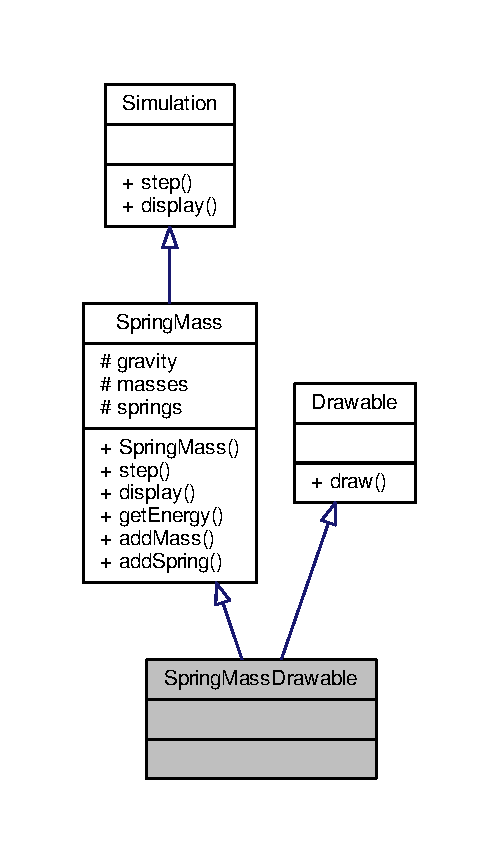
\includegraphics[width=240pt]{classSpringMassDrawable__inherit__graph}
\end{center}
\end{figure}


Collaboration diagram for Spring\+Mass\+Drawable\+:
\nopagebreak
\begin{figure}[H]
\begin{center}
\leavevmode
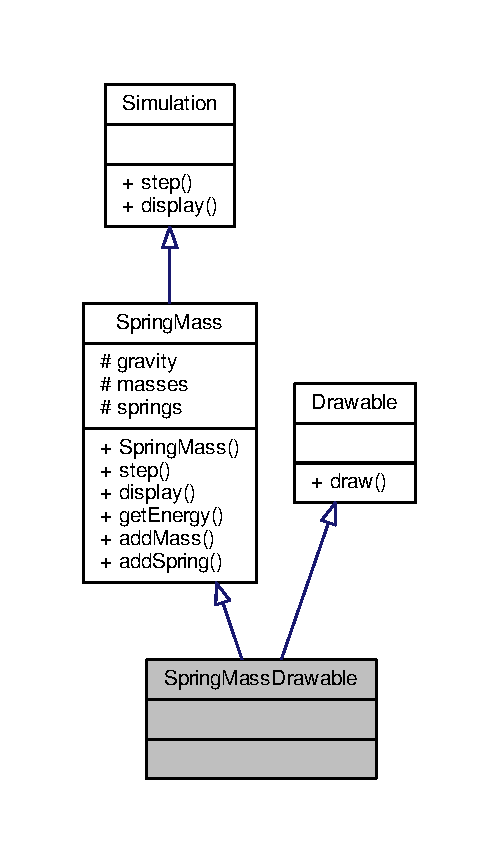
\includegraphics[width=240pt]{classSpringMassDrawable__coll__graph}
\end{center}
\end{figure}
\subsection*{Additional Inherited Members}


\subsection{Detailed Description}
file\+: \hyperlink{test-springmass-graphics_8cpp}{test-\/springmass-\/graphics.\+cpp} brief\+: Tests the spring mass simulation with graphics author\+: Andrea Vedaldi 

The documentation for this class was generated from the following file\+:\begin{DoxyCompactItemize}
\item 
\hyperlink{test-springmass-graphics_8cpp}{test-\/springmass-\/graphics.\+cpp}\end{DoxyCompactItemize}

\hypertarget{classVector2}{}\section{Vector2 Class Reference}
\label{classVector2}\index{Vector2@{Vector2}}


{\ttfamily \#include $<$springmass.\+h$>$}



Collaboration diagram for Vector2\+:
\nopagebreak
\begin{figure}[H]
\begin{center}
\leavevmode
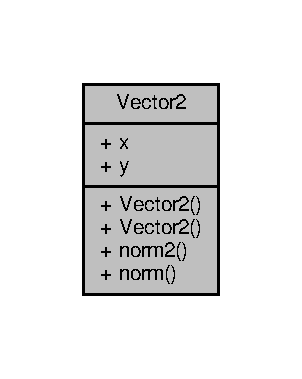
\includegraphics[width=145pt]{classVector2__coll__graph}
\end{center}
\end{figure}
\subsection*{Public Member Functions}
\begin{DoxyCompactItemize}
\item 
\hyperlink{classVector2_a22104d1809be26a419ef1f959e3761bf}{Vector2} ()
\item 
\hyperlink{classVector2_a861062b13bd0e92d50b3ffd90c9edd77}{Vector2} (double \+\_\+x, double \+\_\+y)
\item 
double \hyperlink{classVector2_a08452f15b4693e07c992b77053b24d89}{norm2} () const
\item 
double \hyperlink{classVector2_aa237ac7d74130707d189c3740bc34f94}{norm} () const
\end{DoxyCompactItemize}
\subsection*{Public Attributes}
\begin{DoxyCompactItemize}
\item 
double \hyperlink{classVector2_a61d73d9036ccbb3257fbe595c014a1d0}{x}
\item 
double \hyperlink{classVector2_a4df9b2a8e79e6e30a7a3b34722d8b8b8}{y}
\end{DoxyCompactItemize}


\subsection{Constructor \& Destructor Documentation}
\mbox{\Hypertarget{classVector2_a22104d1809be26a419ef1f959e3761bf}\label{classVector2_a22104d1809be26a419ef1f959e3761bf}} 
\index{Vector2@{Vector2}!Vector2@{Vector2}}
\index{Vector2@{Vector2}!Vector2@{Vector2}}
\subsubsection{\texorpdfstring{Vector2()}{Vector2()}\hspace{0.1cm}{\footnotesize\ttfamily [1/2]}}
{\footnotesize\ttfamily Vector2\+::\+Vector2 (\begin{DoxyParamCaption}{ }\end{DoxyParamCaption})\hspace{0.3cm}{\ttfamily [inline]}}

\mbox{\Hypertarget{classVector2_a861062b13bd0e92d50b3ffd90c9edd77}\label{classVector2_a861062b13bd0e92d50b3ffd90c9edd77}} 
\index{Vector2@{Vector2}!Vector2@{Vector2}}
\index{Vector2@{Vector2}!Vector2@{Vector2}}
\subsubsection{\texorpdfstring{Vector2()}{Vector2()}\hspace{0.1cm}{\footnotesize\ttfamily [2/2]}}
{\footnotesize\ttfamily Vector2\+::\+Vector2 (\begin{DoxyParamCaption}\item[{double}]{\+\_\+x,  }\item[{double}]{\+\_\+y }\end{DoxyParamCaption})\hspace{0.3cm}{\ttfamily [inline]}}



\subsection{Member Function Documentation}
\mbox{\Hypertarget{classVector2_aa237ac7d74130707d189c3740bc34f94}\label{classVector2_aa237ac7d74130707d189c3740bc34f94}} 
\index{Vector2@{Vector2}!norm@{norm}}
\index{norm@{norm}!Vector2@{Vector2}}
\subsubsection{\texorpdfstring{norm()}{norm()}}
{\footnotesize\ttfamily double Vector2\+::norm (\begin{DoxyParamCaption}{ }\end{DoxyParamCaption}) const\hspace{0.3cm}{\ttfamily [inline]}}

\mbox{\Hypertarget{classVector2_a08452f15b4693e07c992b77053b24d89}\label{classVector2_a08452f15b4693e07c992b77053b24d89}} 
\index{Vector2@{Vector2}!norm2@{norm2}}
\index{norm2@{norm2}!Vector2@{Vector2}}
\subsubsection{\texorpdfstring{norm2()}{norm2()}}
{\footnotesize\ttfamily double Vector2\+::norm2 (\begin{DoxyParamCaption}{ }\end{DoxyParamCaption}) const\hspace{0.3cm}{\ttfamily [inline]}}



\subsection{Member Data Documentation}
\mbox{\Hypertarget{classVector2_a61d73d9036ccbb3257fbe595c014a1d0}\label{classVector2_a61d73d9036ccbb3257fbe595c014a1d0}} 
\index{Vector2@{Vector2}!x@{x}}
\index{x@{x}!Vector2@{Vector2}}
\subsubsection{\texorpdfstring{x}{x}}
{\footnotesize\ttfamily double Vector2\+::x}

\mbox{\Hypertarget{classVector2_a4df9b2a8e79e6e30a7a3b34722d8b8b8}\label{classVector2_a4df9b2a8e79e6e30a7a3b34722d8b8b8}} 
\index{Vector2@{Vector2}!y@{y}}
\index{y@{y}!Vector2@{Vector2}}
\subsubsection{\texorpdfstring{y}{y}}
{\footnotesize\ttfamily double Vector2\+::y}



The documentation for this class was generated from the following file\+:\begin{DoxyCompactItemize}
\item 
\hyperlink{springmass_8h}{springmass.\+h}\end{DoxyCompactItemize}

\chapter{File Documentation}
\hypertarget{ball_8cpp}{}\section{ball.\+cpp File Reference}
\label{ball_8cpp}\index{ball.\+cpp@{ball.\+cpp}}
{\ttfamily \#include \char`\"{}ball.\+h\char`\"{}}\newline
{\ttfamily \#include $<$iostream$>$}\newline
Include dependency graph for ball.\+cpp\+:
\nopagebreak
\begin{figure}[H]
\begin{center}
\leavevmode
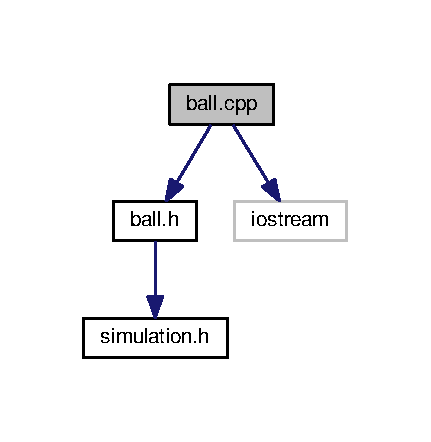
\includegraphics[width=207pt]{ball_8cpp__incl}
\end{center}
\end{figure}

\hypertarget{ball_8h}{}\section{ball.\+h File Reference}
\label{ball_8h}\index{ball.\+h@{ball.\+h}}
{\ttfamily \#include \char`\"{}simulation.\+h\char`\"{}}\newline
Include dependency graph for ball.\+h\+:
\nopagebreak
\begin{figure}[H]
\begin{center}
\leavevmode
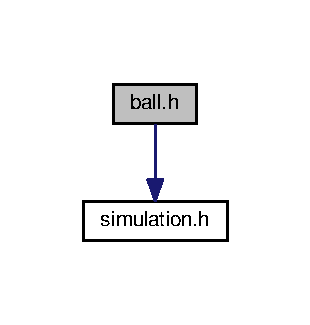
\includegraphics[width=149pt]{ball_8h__incl}
\end{center}
\end{figure}
This graph shows which files directly or indirectly include this file\+:
\nopagebreak
\begin{figure}[H]
\begin{center}
\leavevmode
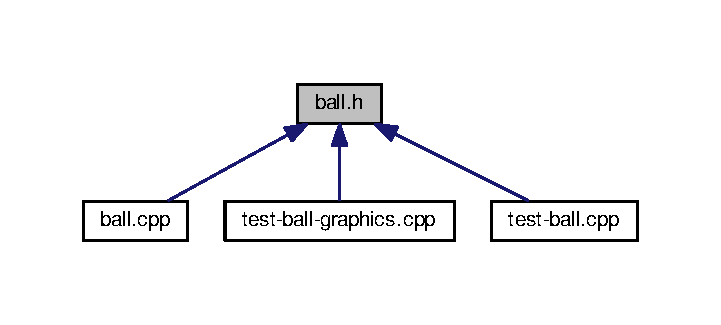
\includegraphics[width=346pt]{ball_8h__dep__incl}
\end{center}
\end{figure}
\subsection*{Classes}
\begin{DoxyCompactItemize}
\item 
class \hyperlink{classBall}{Ball}
\end{DoxyCompactItemize}

\hypertarget{graphics_8cpp}{}\section{graphics.\+cpp File Reference}
\label{graphics_8cpp}\index{graphics.\+cpp@{graphics.\+cpp}}
{\ttfamily \#include \char`\"{}graphics.\+h\char`\"{}}\newline
{\ttfamily \#include $<$cassert$>$}\newline
{\ttfamily \#include $<$cmath$>$}\newline
{\ttfamily \#include $<$iostream$>$}\newline
{\ttfamily \#include $<$algorithm$>$}\newline
{\ttfamily \#include $<$sstream$>$}\newline
{\ttfamily \#include $<$iomanip$>$}\newline
Include dependency graph for graphics.\+cpp\+:
\nopagebreak
\begin{figure}[H]
\begin{center}
\leavevmode
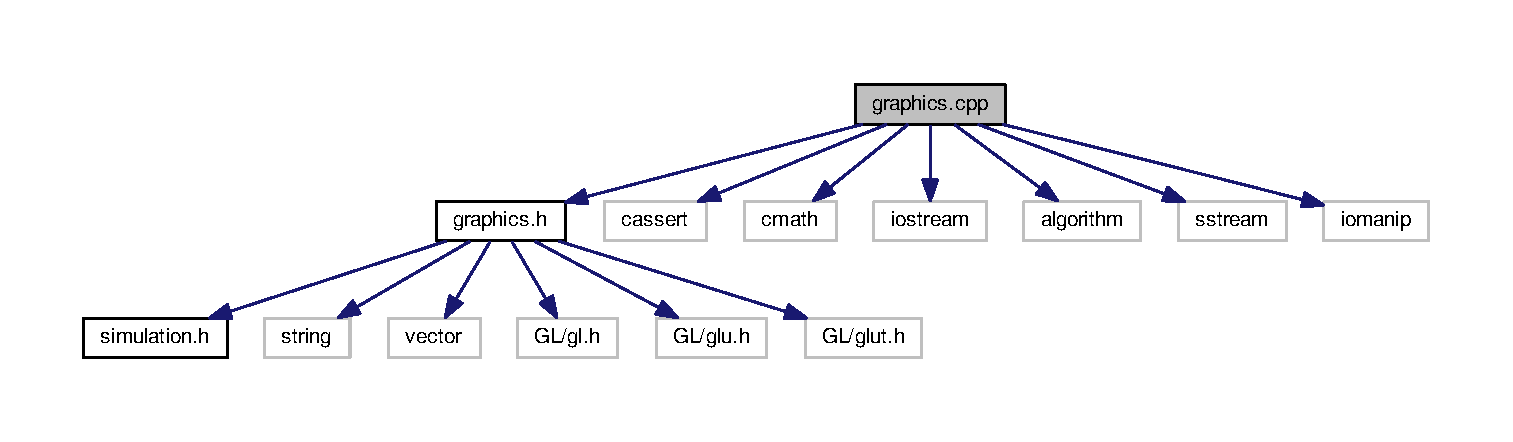
\includegraphics[width=350pt]{graphics_8cpp__incl}
\end{center}
\end{figure}
\subsection*{Typedefs}
\begin{DoxyCompactItemize}
\item 
typedef std\+::vector$<$ \hyperlink{classFigure}{Figure} $\ast$ $>$ \hyperlink{graphics_8cpp_abe02648a451965fae83d1276b6073260}{figures\+\_\+t}
\end{DoxyCompactItemize}
\subsection*{Functions}
\begin{DoxyCompactItemize}
\item 
int \hyperlink{graphics_8cpp_ace3c148657c05d4b13aab34ffef560fe}{R\+O\+U\+ND} (float x)
\item 
void \hyperlink{graphics_8cpp_adcd2119d5c903d502202458acaaa04b1}{handle\+Timer} (int id)
\item 
void \hyperlink{graphics_8cpp_a13a43e6d814de94978c515cb084873b1}{run} ()
\item 
void \hyperlink{graphics_8cpp_a0861523e83bae88b69987cfb79dccbfa}{run} (\hyperlink{classSimulation}{Simulation} $\ast$simulation, double time\+Step)
\end{DoxyCompactItemize}
\subsection*{Variables}
\begin{DoxyCompactItemize}
\item 
\hyperlink{graphics_8cpp_abe02648a451965fae83d1276b6073260}{figures\+\_\+t} \hyperlink{graphics_8cpp_a40a0c0dd97e6a866f089490393685764}{figures}
\item 
\hyperlink{classSimulation}{Simulation} $\ast$ \hyperlink{graphics_8cpp_a041ceee124d1b4999cff56ea55529fbe}{running\+Simulation} = N\+U\+LL
\item 
double \hyperlink{graphics_8cpp_a485f580bc91e4fbdab5c8f1cb080e96f}{running\+Simulation\+Time}
\item 
double \hyperlink{graphics_8cpp_a35d868eb3000aaf61ae8c9a8f84ae532}{running\+Simulation\+Time\+Step}
\end{DoxyCompactItemize}


\subsection{Typedef Documentation}
\mbox{\Hypertarget{graphics_8cpp_abe02648a451965fae83d1276b6073260}\label{graphics_8cpp_abe02648a451965fae83d1276b6073260}} 
\index{graphics.\+cpp@{graphics.\+cpp}!figures\+\_\+t@{figures\+\_\+t}}
\index{figures\+\_\+t@{figures\+\_\+t}!graphics.\+cpp@{graphics.\+cpp}}
\subsubsection{\texorpdfstring{figures\+\_\+t}{figures\_t}}
{\footnotesize\ttfamily typedef std\+::vector$<$\hyperlink{classFigure}{Figure}$\ast$$>$ \hyperlink{graphics_8cpp_abe02648a451965fae83d1276b6073260}{figures\+\_\+t}}



\subsection{Function Documentation}
\mbox{\Hypertarget{graphics_8cpp_adcd2119d5c903d502202458acaaa04b1}\label{graphics_8cpp_adcd2119d5c903d502202458acaaa04b1}} 
\index{graphics.\+cpp@{graphics.\+cpp}!handle\+Timer@{handle\+Timer}}
\index{handle\+Timer@{handle\+Timer}!graphics.\+cpp@{graphics.\+cpp}}
\subsubsection{\texorpdfstring{handle\+Timer()}{handleTimer()}}
{\footnotesize\ttfamily void handle\+Timer (\begin{DoxyParamCaption}\item[{int}]{id }\end{DoxyParamCaption})}

\mbox{\Hypertarget{graphics_8cpp_ace3c148657c05d4b13aab34ffef560fe}\label{graphics_8cpp_ace3c148657c05d4b13aab34ffef560fe}} 
\index{graphics.\+cpp@{graphics.\+cpp}!R\+O\+U\+ND@{R\+O\+U\+ND}}
\index{R\+O\+U\+ND@{R\+O\+U\+ND}!graphics.\+cpp@{graphics.\+cpp}}
\subsubsection{\texorpdfstring{R\+O\+U\+N\+D()}{ROUND()}}
{\footnotesize\ttfamily int R\+O\+U\+ND (\begin{DoxyParamCaption}\item[{float}]{x }\end{DoxyParamCaption})\hspace{0.3cm}{\ttfamily [inline]}}

file\+: \hyperlink{graphics_8cpp}{graphics.\+cpp} brief\+: Graphic helpers implementation author\+: Andrea Vedaldi \mbox{\Hypertarget{graphics_8cpp_a13a43e6d814de94978c515cb084873b1}\label{graphics_8cpp_a13a43e6d814de94978c515cb084873b1}} 
\index{graphics.\+cpp@{graphics.\+cpp}!run@{run}}
\index{run@{run}!graphics.\+cpp@{graphics.\+cpp}}
\subsubsection{\texorpdfstring{run()}{run()}\hspace{0.1cm}{\footnotesize\ttfamily [1/2]}}
{\footnotesize\ttfamily void run (\begin{DoxyParamCaption}{ }\end{DoxyParamCaption})}

file\+: \hyperlink{graphics_8h}{graphics.\+h} brief\+: Graphics helpers author\+: Andrea Vedaldi \mbox{\Hypertarget{graphics_8cpp_a0861523e83bae88b69987cfb79dccbfa}\label{graphics_8cpp_a0861523e83bae88b69987cfb79dccbfa}} 
\index{graphics.\+cpp@{graphics.\+cpp}!run@{run}}
\index{run@{run}!graphics.\+cpp@{graphics.\+cpp}}
\subsubsection{\texorpdfstring{run()}{run()}\hspace{0.1cm}{\footnotesize\ttfamily [2/2]}}
{\footnotesize\ttfamily void run (\begin{DoxyParamCaption}\item[{\hyperlink{classSimulation}{Simulation} $\ast$}]{simulation,  }\item[{double}]{time\+Step }\end{DoxyParamCaption})}



\subsection{Variable Documentation}
\mbox{\Hypertarget{graphics_8cpp_a40a0c0dd97e6a866f089490393685764}\label{graphics_8cpp_a40a0c0dd97e6a866f089490393685764}} 
\index{graphics.\+cpp@{graphics.\+cpp}!figures@{figures}}
\index{figures@{figures}!graphics.\+cpp@{graphics.\+cpp}}
\subsubsection{\texorpdfstring{figures}{figures}}
{\footnotesize\ttfamily \hyperlink{graphics_8cpp_abe02648a451965fae83d1276b6073260}{figures\+\_\+t} figures}

\mbox{\Hypertarget{graphics_8cpp_a041ceee124d1b4999cff56ea55529fbe}\label{graphics_8cpp_a041ceee124d1b4999cff56ea55529fbe}} 
\index{graphics.\+cpp@{graphics.\+cpp}!running\+Simulation@{running\+Simulation}}
\index{running\+Simulation@{running\+Simulation}!graphics.\+cpp@{graphics.\+cpp}}
\subsubsection{\texorpdfstring{running\+Simulation}{runningSimulation}}
{\footnotesize\ttfamily \hyperlink{classSimulation}{Simulation}$\ast$ running\+Simulation = N\+U\+LL}

\mbox{\Hypertarget{graphics_8cpp_a485f580bc91e4fbdab5c8f1cb080e96f}\label{graphics_8cpp_a485f580bc91e4fbdab5c8f1cb080e96f}} 
\index{graphics.\+cpp@{graphics.\+cpp}!running\+Simulation\+Time@{running\+Simulation\+Time}}
\index{running\+Simulation\+Time@{running\+Simulation\+Time}!graphics.\+cpp@{graphics.\+cpp}}
\subsubsection{\texorpdfstring{running\+Simulation\+Time}{runningSimulationTime}}
{\footnotesize\ttfamily double running\+Simulation\+Time}

\mbox{\Hypertarget{graphics_8cpp_a35d868eb3000aaf61ae8c9a8f84ae532}\label{graphics_8cpp_a35d868eb3000aaf61ae8c9a8f84ae532}} 
\index{graphics.\+cpp@{graphics.\+cpp}!running\+Simulation\+Time\+Step@{running\+Simulation\+Time\+Step}}
\index{running\+Simulation\+Time\+Step@{running\+Simulation\+Time\+Step}!graphics.\+cpp@{graphics.\+cpp}}
\subsubsection{\texorpdfstring{running\+Simulation\+Time\+Step}{runningSimulationTimeStep}}
{\footnotesize\ttfamily double running\+Simulation\+Time\+Step}


\hypertarget{graphics_8h}{}\section{graphics.\+h File Reference}
\label{graphics_8h}\index{graphics.\+h@{graphics.\+h}}
{\ttfamily \#include \char`\"{}simulation.\+h\char`\"{}}\newline
{\ttfamily \#include $<$string$>$}\newline
{\ttfamily \#include $<$vector$>$}\newline
{\ttfamily \#include $<$G\+L/gl.\+h$>$}\newline
{\ttfamily \#include $<$G\+L/glu.\+h$>$}\newline
{\ttfamily \#include $<$G\+L/glut.\+h$>$}\newline
Include dependency graph for graphics.\+h\+:
\nopagebreak
\begin{figure}[H]
\begin{center}
\leavevmode
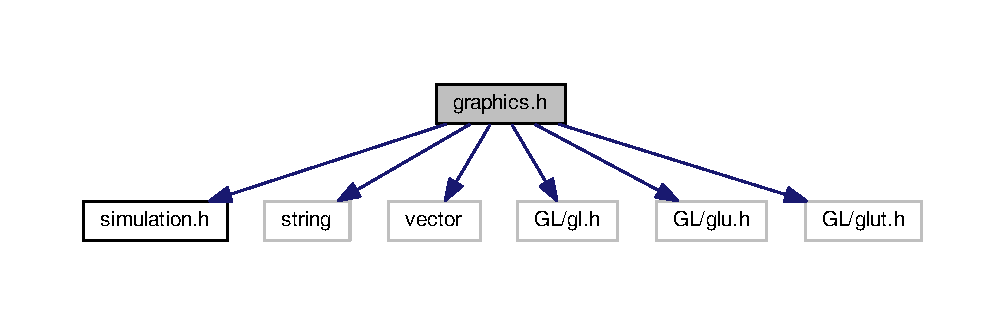
\includegraphics[width=350pt]{graphics_8h__incl}
\end{center}
\end{figure}
This graph shows which files directly or indirectly include this file\+:
\nopagebreak
\begin{figure}[H]
\begin{center}
\leavevmode
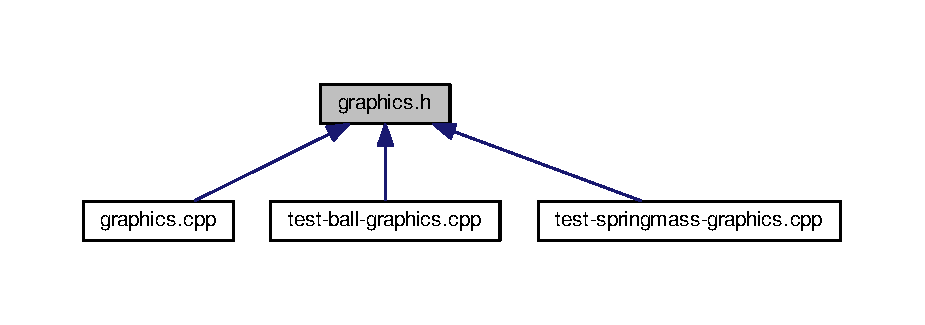
\includegraphics[width=350pt]{graphics_8h__dep__incl}
\end{center}
\end{figure}
\subsection*{Classes}
\begin{DoxyCompactItemize}
\item 
class \hyperlink{classDrawable}{Drawable}
\item 
class \hyperlink{classFigure}{Figure}
\end{DoxyCompactItemize}
\subsection*{Functions}
\begin{DoxyCompactItemize}
\item 
void \hyperlink{graphics_8h_a13a43e6d814de94978c515cb084873b1}{run} ()
\item 
void \hyperlink{graphics_8h_a0861523e83bae88b69987cfb79dccbfa}{run} (\hyperlink{classSimulation}{Simulation} $\ast$simulation, double time\+Step)
\end{DoxyCompactItemize}


\subsection{Function Documentation}
\mbox{\Hypertarget{graphics_8h_a13a43e6d814de94978c515cb084873b1}\label{graphics_8h_a13a43e6d814de94978c515cb084873b1}} 
\index{graphics.\+h@{graphics.\+h}!run@{run}}
\index{run@{run}!graphics.\+h@{graphics.\+h}}
\subsubsection{\texorpdfstring{run()}{run()}\hspace{0.1cm}{\footnotesize\ttfamily [1/2]}}
{\footnotesize\ttfamily void run (\begin{DoxyParamCaption}{ }\end{DoxyParamCaption})}

file\+: \hyperlink{graphics_8h}{graphics.\+h} brief\+: Graphics helpers author\+: Andrea Vedaldi \mbox{\Hypertarget{graphics_8h_a0861523e83bae88b69987cfb79dccbfa}\label{graphics_8h_a0861523e83bae88b69987cfb79dccbfa}} 
\index{graphics.\+h@{graphics.\+h}!run@{run}}
\index{run@{run}!graphics.\+h@{graphics.\+h}}
\subsubsection{\texorpdfstring{run()}{run()}\hspace{0.1cm}{\footnotesize\ttfamily [2/2]}}
{\footnotesize\ttfamily void run (\begin{DoxyParamCaption}\item[{\hyperlink{classSimulation}{Simulation} $\ast$}]{simulation,  }\item[{double}]{time\+Step }\end{DoxyParamCaption})}


\hypertarget{plot__ball_8m}{}\section{plot\+\_\+ball.\+m File Reference}
\label{plot__ball_8m}\index{plot\+\_\+ball.\+m@{plot\+\_\+ball.\+m}}
\subsection*{Functions}
\begin{DoxyCompactItemize}
\item 
\hyperlink{plot__ball_8m_a8cec873ab0d331951a3f7c4efe17237b}{load} (\textquotesingle{}ball.\+txt\textquotesingle{})
\item 
\hyperlink{plot__ball_8m_abb5bf68d8a75c944278f8d8c407200b5}{axis} (\mbox{[}-\/1, 1, -\/1, 0\mbox{]}) for c
\item 
\hyperlink{plot__ball_8m_ae7ade489d6745c00227faf5e7fb1ec68}{plot} (ball(c, 1), ball(c, 2), \textquotesingle{}o\textquotesingle{}, \textquotesingle{}Marker\+Size\textquotesingle{}, 20, \textquotesingle{}Line\+Width\textquotesingle{}, 5)
\end{DoxyCompactItemize}
\subsection*{Variables}
\begin{DoxyCompactItemize}
\item 
\hyperlink{plot__ball_8m_a391e34f2de441d79152a7b3d6e4c9c86}{figure}
\item 
hold \hyperlink{plot__ball_8m_a58ab1fd68e97078232808206b850161b}{on}
\end{DoxyCompactItemize}


\subsection{Function Documentation}
\mbox{\Hypertarget{plot__ball_8m_abb5bf68d8a75c944278f8d8c407200b5}\label{plot__ball_8m_abb5bf68d8a75c944278f8d8c407200b5}} 
\index{plot\+\_\+ball.\+m@{plot\+\_\+ball.\+m}!axis@{axis}}
\index{axis@{axis}!plot\+\_\+ball.\+m@{plot\+\_\+ball.\+m}}
\subsubsection{\texorpdfstring{axis()}{axis()}}
{\footnotesize\ttfamily axis (\begin{DoxyParamCaption}{ }\end{DoxyParamCaption})}

\mbox{\Hypertarget{plot__ball_8m_a8cec873ab0d331951a3f7c4efe17237b}\label{plot__ball_8m_a8cec873ab0d331951a3f7c4efe17237b}} 
\index{plot\+\_\+ball.\+m@{plot\+\_\+ball.\+m}!load@{load}}
\index{load@{load}!plot\+\_\+ball.\+m@{plot\+\_\+ball.\+m}}
\subsubsection{\texorpdfstring{load()}{load()}}
{\footnotesize\ttfamily load (\begin{DoxyParamCaption}\item[{\textquotesingle{}ball.\+txt\textquotesingle{}}]{ }\end{DoxyParamCaption})}

\mbox{\Hypertarget{plot__ball_8m_ae7ade489d6745c00227faf5e7fb1ec68}\label{plot__ball_8m_ae7ade489d6745c00227faf5e7fb1ec68}} 
\index{plot\+\_\+ball.\+m@{plot\+\_\+ball.\+m}!plot@{plot}}
\index{plot@{plot}!plot\+\_\+ball.\+m@{plot\+\_\+ball.\+m}}
\subsubsection{\texorpdfstring{plot()}{plot()}}
{\footnotesize\ttfamily plot (\begin{DoxyParamCaption}\item[{ball(c, 1)}]{,  }\item[{ball(c, 2)}]{,  }\item[{\textquotesingle{}o\textquotesingle{}}]{,  }\item[{\textquotesingle{}Marker\+Size\textquotesingle{}}]{,  }\item[{20}]{,  }\item[{\textquotesingle{}Line\+Width\textquotesingle{}}]{,  }\item[{5}]{ }\end{DoxyParamCaption})}



\subsection{Variable Documentation}
\mbox{\Hypertarget{plot__ball_8m_a391e34f2de441d79152a7b3d6e4c9c86}\label{plot__ball_8m_a391e34f2de441d79152a7b3d6e4c9c86}} 
\index{plot\+\_\+ball.\+m@{plot\+\_\+ball.\+m}!figure@{figure}}
\index{figure@{figure}!plot\+\_\+ball.\+m@{plot\+\_\+ball.\+m}}
\subsubsection{\texorpdfstring{figure}{figure}}
{\footnotesize\ttfamily figure}

\mbox{\Hypertarget{plot__ball_8m_a58ab1fd68e97078232808206b850161b}\label{plot__ball_8m_a58ab1fd68e97078232808206b850161b}} 
\index{plot\+\_\+ball.\+m@{plot\+\_\+ball.\+m}!on@{on}}
\index{on@{on}!plot\+\_\+ball.\+m@{plot\+\_\+ball.\+m}}
\subsubsection{\texorpdfstring{on}{on}}
{\footnotesize\ttfamily hold on}


\hypertarget{README_8md}{}\section{R\+E\+A\+D\+M\+E.\+md File Reference}
\label{README_8md}\index{R\+E\+A\+D\+M\+E.\+md@{R\+E\+A\+D\+M\+E.\+md}}

\hypertarget{simulation_8h}{}\section{simulation.\+h File Reference}
\label{simulation_8h}\index{simulation.\+h@{simulation.\+h}}
This graph shows which files directly or indirectly include this file\+:
\nopagebreak
\begin{figure}[H]
\begin{center}
\leavevmode
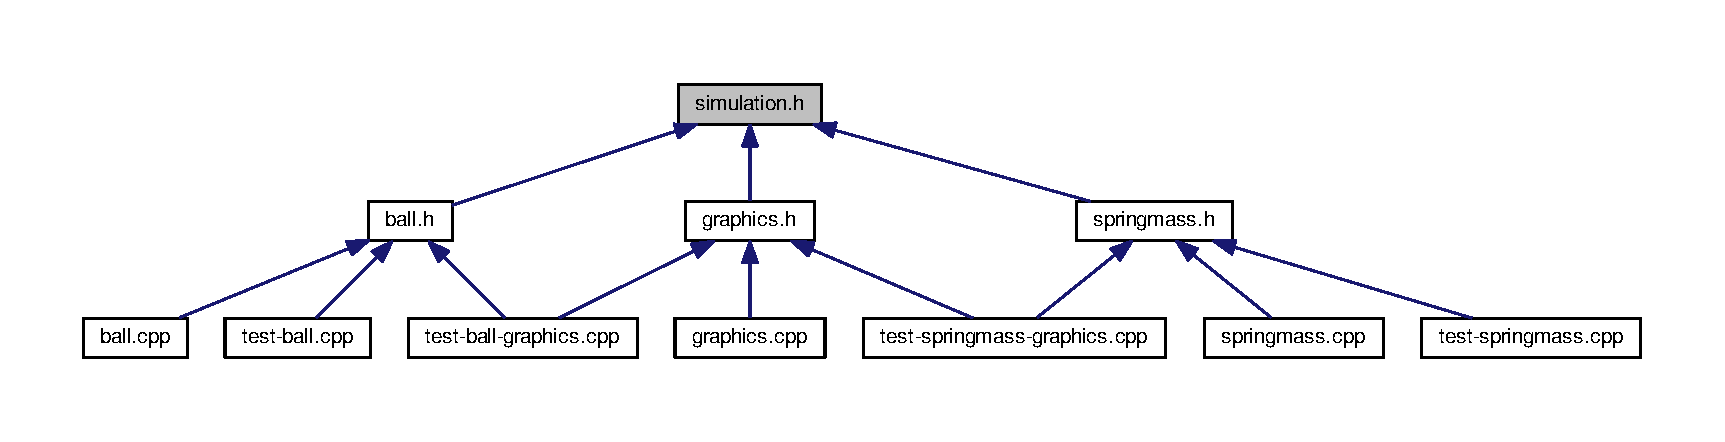
\includegraphics[width=350pt]{simulation_8h__dep__incl}
\end{center}
\end{figure}
\subsection*{Classes}
\begin{DoxyCompactItemize}
\item 
class \hyperlink{classSimulation}{Simulation}
\end{DoxyCompactItemize}

\hypertarget{springmass_8cpp}{}\section{springmass.\+cpp File Reference}
\label{springmass_8cpp}\index{springmass.\+cpp@{springmass.\+cpp}}
{\ttfamily \#include \char`\"{}springmass.\+h\char`\"{}}\newline
{\ttfamily \#include $<$iostream$>$}\newline
Include dependency graph for springmass.\+cpp\+:
\nopagebreak
\begin{figure}[H]
\begin{center}
\leavevmode
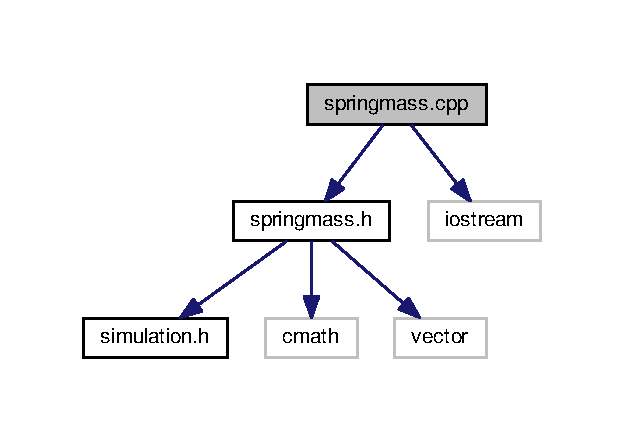
\includegraphics[width=300pt]{springmass_8cpp__incl}
\end{center}
\end{figure}
\subsection*{Functions}
\begin{DoxyCompactItemize}
\item 
std\+::ostream \& \hyperlink{springmass_8cpp_a0f7d372af30dcada3c8d4c73d3cfdbe7}{operator$<$$<$} (std\+::ostream \&os, const \hyperlink{classMass}{Mass} \&m)
\item 
std\+::ostream \& \hyperlink{springmass_8cpp_a4529db441fab51d6df9a29216a22ee97}{operator$<$$<$} (std\+::ostream \&os, const \hyperlink{classSpring}{Spring} \&s)
\end{DoxyCompactItemize}


\subsection{Function Documentation}
\mbox{\Hypertarget{springmass_8cpp_a0f7d372af30dcada3c8d4c73d3cfdbe7}\label{springmass_8cpp_a0f7d372af30dcada3c8d4c73d3cfdbe7}} 
\index{springmass.\+cpp@{springmass.\+cpp}!operator$<$$<$@{operator$<$$<$}}
\index{operator$<$$<$@{operator$<$$<$}!springmass.\+cpp@{springmass.\+cpp}}
\subsubsection{\texorpdfstring{operator$<$$<$()}{operator<<()}\hspace{0.1cm}{\footnotesize\ttfamily [1/2]}}
{\footnotesize\ttfamily std\+::ostream\& operator$<$$<$ (\begin{DoxyParamCaption}\item[{std\+::ostream \&}]{os,  }\item[{const \hyperlink{classMass}{Mass} \&}]{m }\end{DoxyParamCaption})}

\mbox{\Hypertarget{springmass_8cpp_a4529db441fab51d6df9a29216a22ee97}\label{springmass_8cpp_a4529db441fab51d6df9a29216a22ee97}} 
\index{springmass.\+cpp@{springmass.\+cpp}!operator$<$$<$@{operator$<$$<$}}
\index{operator$<$$<$@{operator$<$$<$}!springmass.\+cpp@{springmass.\+cpp}}
\subsubsection{\texorpdfstring{operator$<$$<$()}{operator<<()}\hspace{0.1cm}{\footnotesize\ttfamily [2/2]}}
{\footnotesize\ttfamily std\+::ostream\& operator$<$$<$ (\begin{DoxyParamCaption}\item[{std\+::ostream \&}]{os,  }\item[{const \hyperlink{classSpring}{Spring} \&}]{s }\end{DoxyParamCaption})}


\hypertarget{springmass_8h}{}\section{springmass.\+h File Reference}
\label{springmass_8h}\index{springmass.\+h@{springmass.\+h}}
{\ttfamily \#include \char`\"{}simulation.\+h\char`\"{}}\newline
{\ttfamily \#include $<$cmath$>$}\newline
{\ttfamily \#include $<$vector$>$}\newline
Include dependency graph for springmass.\+h\+:
\nopagebreak
\begin{figure}[H]
\begin{center}
\leavevmode
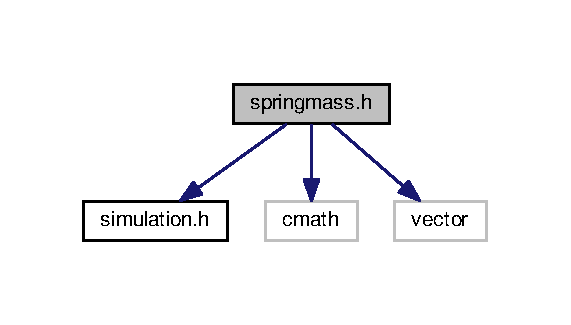
\includegraphics[width=274pt]{springmass_8h__incl}
\end{center}
\end{figure}
This graph shows which files directly or indirectly include this file\+:
\nopagebreak
\begin{figure}[H]
\begin{center}
\leavevmode
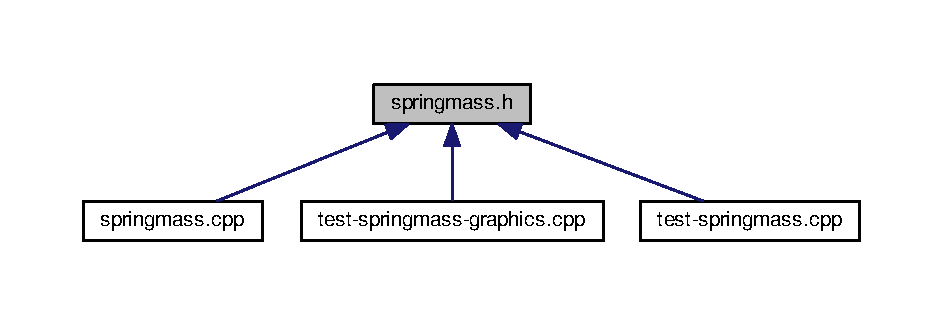
\includegraphics[width=350pt]{springmass_8h__dep__incl}
\end{center}
\end{figure}
\subsection*{Classes}
\begin{DoxyCompactItemize}
\item 
class \hyperlink{classVector2}{Vector2}
\item 
class \hyperlink{classMass}{Mass}
\item 
class \hyperlink{classSpring}{Spring}
\item 
class \hyperlink{classSpringMass}{Spring\+Mass}
\end{DoxyCompactItemize}
\subsection*{Macros}
\begin{DoxyCompactItemize}
\item 
\#define \hyperlink{springmass_8h_a03ad3bae72a0ac7965460a63fd454f44}{M\+O\+O\+N\+\_\+\+G\+R\+A\+V\+I\+TY}~1.\+62
\item 
\#define \hyperlink{springmass_8h_a86d8ad802eb726f5cef184892a3b45a4}{E\+A\+R\+T\+H\+\_\+\+G\+R\+A\+V\+I\+TY}~9.\+82
\end{DoxyCompactItemize}
\subsection*{Functions}
\begin{DoxyCompactItemize}
\item 
\hyperlink{classVector2}{Vector2} \hyperlink{springmass_8h_a31e3edd3b25d0dfe3b9a0b07e93f3365}{operator+} (\hyperlink{classVector2}{Vector2} a, \hyperlink{classVector2}{Vector2} b)
\item 
\hyperlink{classVector2}{Vector2} \hyperlink{springmass_8h_a1a3d5fba2778a3d4c97629baca753853}{operator-\/} (\hyperlink{classVector2}{Vector2} a, \hyperlink{classVector2}{Vector2} b)
\item 
\hyperlink{classVector2}{Vector2} \hyperlink{springmass_8h_a28a37cea996dfa0b6d7c048ac89227bb}{operator$\ast$} (double a, \hyperlink{classVector2}{Vector2} b)
\item 
\hyperlink{classVector2}{Vector2} \hyperlink{springmass_8h_a3e6ab2ac27cc68b574eaea146bd714ce}{operator$\ast$} (\hyperlink{classVector2}{Vector2} a, double b)
\item 
\hyperlink{classVector2}{Vector2} \hyperlink{springmass_8h_a8f77c1d121d92271c1c736e7b9a38a93}{operator/} (\hyperlink{classVector2}{Vector2} a, double b)
\item 
double \hyperlink{springmass_8h_a6e6659dcf321b29ea4f0f9e763d502d0}{dot} (\hyperlink{classVector2}{Vector2} a, \hyperlink{classVector2}{Vector2} b)
\end{DoxyCompactItemize}


\subsection{Macro Definition Documentation}
\mbox{\Hypertarget{springmass_8h_a86d8ad802eb726f5cef184892a3b45a4}\label{springmass_8h_a86d8ad802eb726f5cef184892a3b45a4}} 
\index{springmass.\+h@{springmass.\+h}!E\+A\+R\+T\+H\+\_\+\+G\+R\+A\+V\+I\+TY@{E\+A\+R\+T\+H\+\_\+\+G\+R\+A\+V\+I\+TY}}
\index{E\+A\+R\+T\+H\+\_\+\+G\+R\+A\+V\+I\+TY@{E\+A\+R\+T\+H\+\_\+\+G\+R\+A\+V\+I\+TY}!springmass.\+h@{springmass.\+h}}
\subsubsection{\texorpdfstring{E\+A\+R\+T\+H\+\_\+\+G\+R\+A\+V\+I\+TY}{EARTH\_GRAVITY}}
{\footnotesize\ttfamily \#define E\+A\+R\+T\+H\+\_\+\+G\+R\+A\+V\+I\+TY~9.\+82}

\mbox{\Hypertarget{springmass_8h_a03ad3bae72a0ac7965460a63fd454f44}\label{springmass_8h_a03ad3bae72a0ac7965460a63fd454f44}} 
\index{springmass.\+h@{springmass.\+h}!M\+O\+O\+N\+\_\+\+G\+R\+A\+V\+I\+TY@{M\+O\+O\+N\+\_\+\+G\+R\+A\+V\+I\+TY}}
\index{M\+O\+O\+N\+\_\+\+G\+R\+A\+V\+I\+TY@{M\+O\+O\+N\+\_\+\+G\+R\+A\+V\+I\+TY}!springmass.\+h@{springmass.\+h}}
\subsubsection{\texorpdfstring{M\+O\+O\+N\+\_\+\+G\+R\+A\+V\+I\+TY}{MOON\_GRAVITY}}
{\footnotesize\ttfamily \#define M\+O\+O\+N\+\_\+\+G\+R\+A\+V\+I\+TY~1.\+62}

file\+: \hyperlink{springmass_8h}{springmass.\+h} brief\+: \hyperlink{classSpringMass}{Spring\+Mass} simulation author\+: Andrea Vedaldi 

\subsection{Function Documentation}
\mbox{\Hypertarget{springmass_8h_a6e6659dcf321b29ea4f0f9e763d502d0}\label{springmass_8h_a6e6659dcf321b29ea4f0f9e763d502d0}} 
\index{springmass.\+h@{springmass.\+h}!dot@{dot}}
\index{dot@{dot}!springmass.\+h@{springmass.\+h}}
\subsubsection{\texorpdfstring{dot()}{dot()}}
{\footnotesize\ttfamily double dot (\begin{DoxyParamCaption}\item[{\hyperlink{classVector2}{Vector2}}]{a,  }\item[{\hyperlink{classVector2}{Vector2}}]{b }\end{DoxyParamCaption})\hspace{0.3cm}{\ttfamily [inline]}}

\mbox{\Hypertarget{springmass_8h_a28a37cea996dfa0b6d7c048ac89227bb}\label{springmass_8h_a28a37cea996dfa0b6d7c048ac89227bb}} 
\index{springmass.\+h@{springmass.\+h}!operator$\ast$@{operator$\ast$}}
\index{operator$\ast$@{operator$\ast$}!springmass.\+h@{springmass.\+h}}
\subsubsection{\texorpdfstring{operator$\ast$()}{operator*()}\hspace{0.1cm}{\footnotesize\ttfamily [1/2]}}
{\footnotesize\ttfamily \hyperlink{classVector2}{Vector2} operator$\ast$ (\begin{DoxyParamCaption}\item[{double}]{a,  }\item[{\hyperlink{classVector2}{Vector2}}]{b }\end{DoxyParamCaption})\hspace{0.3cm}{\ttfamily [inline]}}

\mbox{\Hypertarget{springmass_8h_a3e6ab2ac27cc68b574eaea146bd714ce}\label{springmass_8h_a3e6ab2ac27cc68b574eaea146bd714ce}} 
\index{springmass.\+h@{springmass.\+h}!operator$\ast$@{operator$\ast$}}
\index{operator$\ast$@{operator$\ast$}!springmass.\+h@{springmass.\+h}}
\subsubsection{\texorpdfstring{operator$\ast$()}{operator*()}\hspace{0.1cm}{\footnotesize\ttfamily [2/2]}}
{\footnotesize\ttfamily \hyperlink{classVector2}{Vector2} operator$\ast$ (\begin{DoxyParamCaption}\item[{\hyperlink{classVector2}{Vector2}}]{a,  }\item[{double}]{b }\end{DoxyParamCaption})\hspace{0.3cm}{\ttfamily [inline]}}

\mbox{\Hypertarget{springmass_8h_a31e3edd3b25d0dfe3b9a0b07e93f3365}\label{springmass_8h_a31e3edd3b25d0dfe3b9a0b07e93f3365}} 
\index{springmass.\+h@{springmass.\+h}!operator+@{operator+}}
\index{operator+@{operator+}!springmass.\+h@{springmass.\+h}}
\subsubsection{\texorpdfstring{operator+()}{operator+()}}
{\footnotesize\ttfamily \hyperlink{classVector2}{Vector2} operator+ (\begin{DoxyParamCaption}\item[{\hyperlink{classVector2}{Vector2}}]{a,  }\item[{\hyperlink{classVector2}{Vector2}}]{b }\end{DoxyParamCaption})\hspace{0.3cm}{\ttfamily [inline]}}

\mbox{\Hypertarget{springmass_8h_a1a3d5fba2778a3d4c97629baca753853}\label{springmass_8h_a1a3d5fba2778a3d4c97629baca753853}} 
\index{springmass.\+h@{springmass.\+h}!operator-\/@{operator-\/}}
\index{operator-\/@{operator-\/}!springmass.\+h@{springmass.\+h}}
\subsubsection{\texorpdfstring{operator-\/()}{operator-()}}
{\footnotesize\ttfamily \hyperlink{classVector2}{Vector2} operator-\/ (\begin{DoxyParamCaption}\item[{\hyperlink{classVector2}{Vector2}}]{a,  }\item[{\hyperlink{classVector2}{Vector2}}]{b }\end{DoxyParamCaption})\hspace{0.3cm}{\ttfamily [inline]}}

\mbox{\Hypertarget{springmass_8h_a8f77c1d121d92271c1c736e7b9a38a93}\label{springmass_8h_a8f77c1d121d92271c1c736e7b9a38a93}} 
\index{springmass.\+h@{springmass.\+h}!operator/@{operator/}}
\index{operator/@{operator/}!springmass.\+h@{springmass.\+h}}
\subsubsection{\texorpdfstring{operator/()}{operator/()}}
{\footnotesize\ttfamily \hyperlink{classVector2}{Vector2} operator/ (\begin{DoxyParamCaption}\item[{\hyperlink{classVector2}{Vector2}}]{a,  }\item[{double}]{b }\end{DoxyParamCaption})\hspace{0.3cm}{\ttfamily [inline]}}


\hypertarget{test-ball-graphics_8cpp}{}\section{test-\/ball-\/graphics.cpp File Reference}
\label{test-ball-graphics_8cpp}\index{test-\/ball-\/graphics.\+cpp@{test-\/ball-\/graphics.\+cpp}}
{\ttfamily \#include \char`\"{}graphics.\+h\char`\"{}}\newline
{\ttfamily \#include \char`\"{}ball.\+h\char`\"{}}\newline
{\ttfamily \#include $<$iostream$>$}\newline
{\ttfamily \#include $<$sstream$>$}\newline
{\ttfamily \#include $<$iomanip$>$}\newline
Include dependency graph for test-\/ball-\/graphics.cpp\+:
\nopagebreak
\begin{figure}[H]
\begin{center}
\leavevmode
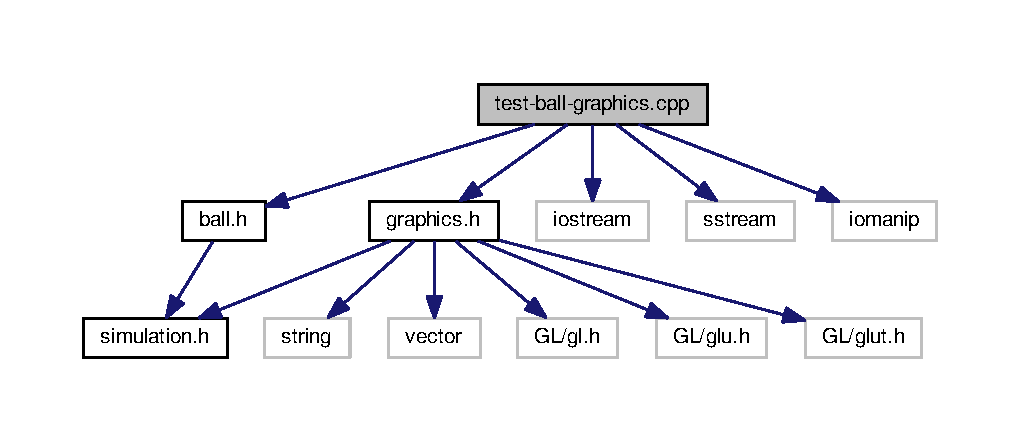
\includegraphics[width=350pt]{test-ball-graphics_8cpp__incl}
\end{center}
\end{figure}
\subsection*{Classes}
\begin{DoxyCompactItemize}
\item 
class \hyperlink{classBallDrawable}{Ball\+Drawable}
\end{DoxyCompactItemize}
\subsection*{Functions}
\begin{DoxyCompactItemize}
\item 
int \hyperlink{test-ball-graphics_8cpp_a3c04138a5bfe5d72780bb7e82a18e627}{main} (int argc, char $\ast$$\ast$argv)
\end{DoxyCompactItemize}


\subsection{Function Documentation}
\mbox{\Hypertarget{test-ball-graphics_8cpp_a3c04138a5bfe5d72780bb7e82a18e627}\label{test-ball-graphics_8cpp_a3c04138a5bfe5d72780bb7e82a18e627}} 
\index{test-\/ball-\/graphics.\+cpp@{test-\/ball-\/graphics.\+cpp}!main@{main}}
\index{main@{main}!test-\/ball-\/graphics.\+cpp@{test-\/ball-\/graphics.\+cpp}}
\subsubsection{\texorpdfstring{main()}{main()}}
{\footnotesize\ttfamily int main (\begin{DoxyParamCaption}\item[{int}]{argc,  }\item[{char $\ast$$\ast$}]{argv }\end{DoxyParamCaption})}


\hypertarget{test-ball_8cpp}{}\section{test-\/ball.cpp File Reference}
\label{test-ball_8cpp}\index{test-\/ball.\+cpp@{test-\/ball.\+cpp}}
{\ttfamily \#include $<$iostream$>$}\newline
{\ttfamily \#include \char`\"{}ball.\+h\char`\"{}}\newline
Include dependency graph for test-\/ball.cpp\+:
\nopagebreak
\begin{figure}[H]
\begin{center}
\leavevmode
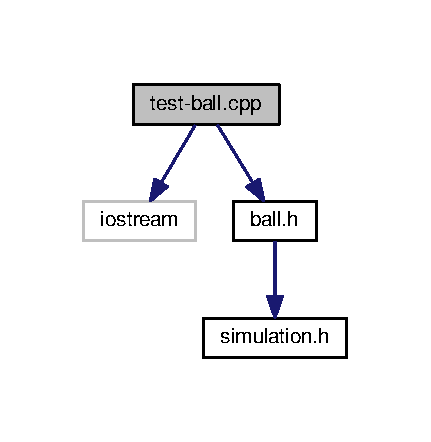
\includegraphics[width=207pt]{test-ball_8cpp__incl}
\end{center}
\end{figure}
\subsection*{Functions}
\begin{DoxyCompactItemize}
\item 
int \hyperlink{test-ball_8cpp_a3c04138a5bfe5d72780bb7e82a18e627}{main} (int argc, char $\ast$$\ast$argv)
\end{DoxyCompactItemize}


\subsection{Function Documentation}
\mbox{\Hypertarget{test-ball_8cpp_a3c04138a5bfe5d72780bb7e82a18e627}\label{test-ball_8cpp_a3c04138a5bfe5d72780bb7e82a18e627}} 
\index{test-\/ball.\+cpp@{test-\/ball.\+cpp}!main@{main}}
\index{main@{main}!test-\/ball.\+cpp@{test-\/ball.\+cpp}}
\subsubsection{\texorpdfstring{main()}{main()}}
{\footnotesize\ttfamily int main (\begin{DoxyParamCaption}\item[{int}]{argc,  }\item[{char $\ast$$\ast$}]{argv }\end{DoxyParamCaption})}


\hypertarget{test-springmass-graphics_8cpp}{}\section{test-\/springmass-\/graphics.cpp File Reference}
\label{test-springmass-graphics_8cpp}\index{test-\/springmass-\/graphics.\+cpp@{test-\/springmass-\/graphics.\+cpp}}
{\ttfamily \#include \char`\"{}graphics.\+h\char`\"{}}\newline
{\ttfamily \#include \char`\"{}springmass.\+h\char`\"{}}\newline
{\ttfamily \#include $<$iostream$>$}\newline
{\ttfamily \#include $<$sstream$>$}\newline
{\ttfamily \#include $<$iomanip$>$}\newline
Include dependency graph for test-\/springmass-\/graphics.cpp\+:
\nopagebreak
\begin{figure}[H]
\begin{center}
\leavevmode
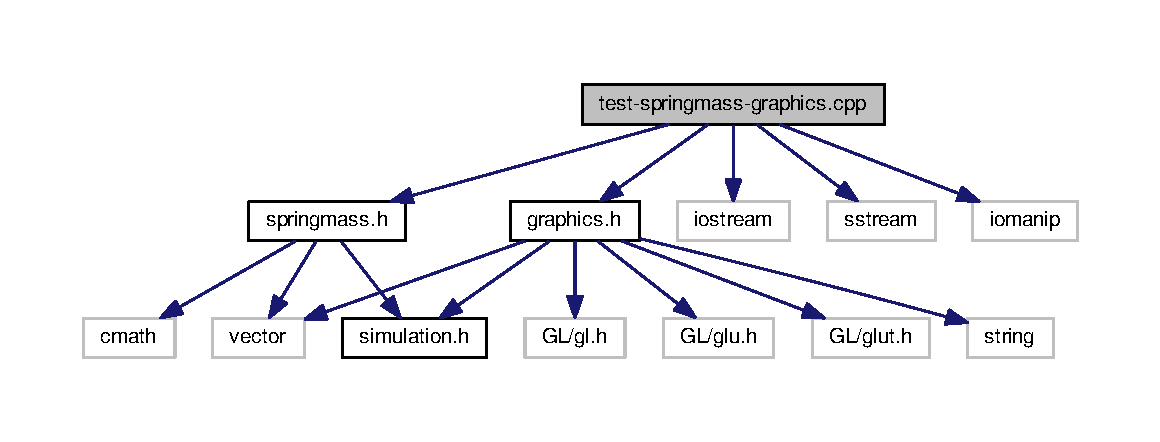
\includegraphics[width=350pt]{test-springmass-graphics_8cpp__incl}
\end{center}
\end{figure}
\subsection*{Classes}
\begin{DoxyCompactItemize}
\item 
class \hyperlink{classSpringMassDrawable}{Spring\+Mass\+Drawable}
\end{DoxyCompactItemize}
\subsection*{Functions}
\begin{DoxyCompactItemize}
\item 
int \hyperlink{test-springmass-graphics_8cpp_a3c04138a5bfe5d72780bb7e82a18e627}{main} (int argc, char $\ast$$\ast$argv)
\end{DoxyCompactItemize}


\subsection{Function Documentation}
\mbox{\Hypertarget{test-springmass-graphics_8cpp_a3c04138a5bfe5d72780bb7e82a18e627}\label{test-springmass-graphics_8cpp_a3c04138a5bfe5d72780bb7e82a18e627}} 
\index{test-\/springmass-\/graphics.\+cpp@{test-\/springmass-\/graphics.\+cpp}!main@{main}}
\index{main@{main}!test-\/springmass-\/graphics.\+cpp@{test-\/springmass-\/graphics.\+cpp}}
\subsubsection{\texorpdfstring{main()}{main()}}
{\footnotesize\ttfamily int main (\begin{DoxyParamCaption}\item[{int}]{argc,  }\item[{char $\ast$$\ast$}]{argv }\end{DoxyParamCaption})}


\hypertarget{test-springmass_8cpp}{}\section{test-\/springmass.cpp File Reference}
\label{test-springmass_8cpp}\index{test-\/springmass.\+cpp@{test-\/springmass.\+cpp}}
{\ttfamily \#include \char`\"{}springmass.\+h\char`\"{}}\newline
Include dependency graph for test-\/springmass.cpp\+:
\nopagebreak
\begin{figure}[H]
\begin{center}
\leavevmode
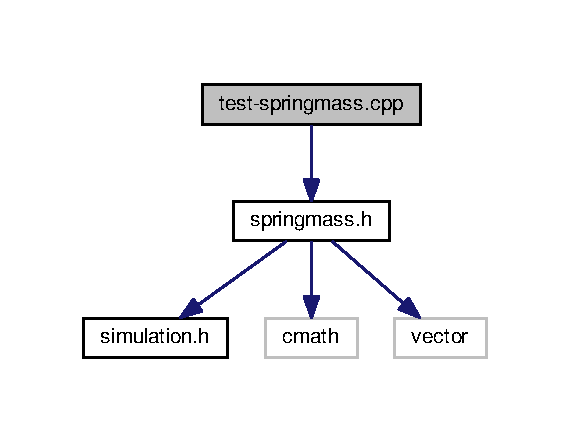
\includegraphics[width=274pt]{test-springmass_8cpp__incl}
\end{center}
\end{figure}
\subsection*{Functions}
\begin{DoxyCompactItemize}
\item 
int \hyperlink{test-springmass_8cpp_a3c04138a5bfe5d72780bb7e82a18e627}{main} (int argc, char $\ast$$\ast$argv)
\end{DoxyCompactItemize}


\subsection{Function Documentation}
\mbox{\Hypertarget{test-springmass_8cpp_a3c04138a5bfe5d72780bb7e82a18e627}\label{test-springmass_8cpp_a3c04138a5bfe5d72780bb7e82a18e627}} 
\index{test-\/springmass.\+cpp@{test-\/springmass.\+cpp}!main@{main}}
\index{main@{main}!test-\/springmass.\+cpp@{test-\/springmass.\+cpp}}
\subsubsection{\texorpdfstring{main()}{main()}}
{\footnotesize\ttfamily int main (\begin{DoxyParamCaption}\item[{int}]{argc,  }\item[{char $\ast$$\ast$}]{argv }\end{DoxyParamCaption})}

file\+: test-\/srpingmass.\+cpp brief\+: Tests the spring mass simulation author\+: Andrea Vedaldi 
%--- End generated contents ---

% Index
\backmatter
\newpage
\phantomsection
\clearemptydoublepage
\addcontentsline{toc}{chapter}{Index}
\printindex

\end{document}
